%%%%%%%%%%%%%%%%%%%%%%%%%%%%%%%%%%%%%%%%%
% Beamer Presentation
% LaTeX Template
% Version 1.0 (10/11/12)
%
% This template has been downloaded from:
% http://www.LaTeXTemplates.com
%
% License:
% CC BY-NC-SA 3.0 (http://creativecommons.org/licenses/by-nc-sa/3.0/)
%
%%%%%%%%%%%%%%%%%%%%%%%%%%%%%%%%%%%%%%%%%

%----------------------------------------------------------------------------------------
%	PACKAGES AND THEMES
%----------------------------------------------------------------------------------------

\documentclass{beamer}

\mode<presentation> {

% The Beamer class comes with a number of default slide themes
% which change the colors and layouts of slides. Below this is a list
% of all the themes, uncomment each in turn to see what they look like.

%\usetheme{default}
%\usetheme{AnnArbor}
%\usetheme{Antibes}
%\usetheme{Bergen}
%\usetheme{Berkeley}
%\usetheme{Berlin}
%\usetheme{Boadilla}
%\usetheme{CambridgeUS}
%\usetheme{Copenhagen}
%\usetheme{Darmstadt}
%\usetheme{Dresden}
%\usetheme{Frankfurt}
%\usetheme{Goettingen}
%\usetheme{Hannover}
%\usetheme{Ilmenau}
%\usetheme{JuanLesPins}
%\usetheme{Luebeck}
\usetheme{Madrid}
%\usetheme{Malmoe}
%\usetheme{Marburg}
%\usetheme{Montpellier}
%\usetheme{PaloAlto}
%\usetheme{Pittsburgh}
%\usetheme{Rochester}
%\usetheme{Singapore}
%\usetheme{Szeged}
%\usetheme{Warsaw}

% As well as themes, the Beamer class has a number of color themes
% for any slide theme. Uncomment each of these in turn to see how it
% changes the colors of your current slide theme.

%\usecolortheme{albatross}
%\usecolortheme{beaver}
%\usecolortheme{beetle}
%\usecolortheme{crane}
\usecolortheme{dolphin}
%\usecolortheme{dove}
%\usecolortheme{fly}
%\usecolortheme{lily}
%\usecolortheme{orchid}
%\usecolortheme{rose}
%\usecolortheme{seagull}
%\usecolortheme{seahorse}
%\usecolortheme{whale}
%\usecolortheme{wolverine}

%\setbeamertemplate{footline} % To remove the footer line in all slides uncomment this line
%\setbeamertemplate{footline}[page number] % To replace the footer line in all slides with a simple slide count uncomment this line

%\setbeamertemplate{navigation symbols}{} % To remove the navigation symbols from the bottom of all slides uncomment this line
}

\usepackage{graphicx} % Allows including images
\usepackage{booktabs} % Allows the use of \toprule, \midrule and \bottomrule in tables
\usepackage{array}
\usepackage{tabularx}
\usepackage[backend=biber,style=apa]{biblatex}
\addbibresource{references.bib}
\usepackage{hyperref}
\usepackage{changepage}
\usepackage[normalem]{ulem}
\hypersetup{
	colorlinks,
    citecolor={blue!70!black},
	linkcolor={blue!70!black},
	urlcolor={blue!70!black}}

\usepackage{appendixnumberbeamer}

%\setbeamercolor{alerted text}{fg=red!70!black}    % warm alert
%\setbeamercolor{alerted text}{fg=orange!80!black} % another option
%\setbeamercolor{alerted text}{fg=cyan!60!black} 

\definecolor{AlertOrangeRed}{RGB}{255,69,0}
\definecolor{AlertDarkOrange}{RGB}{255,140,0}
\definecolor{AlertTomato}{RGB}{255,99,71}
\definecolor{AlertCoral}{RGB}{255,127,80}
\definecolor{AlertGold}{RGB}{255,215,0}
\definecolor{AlertYellowOrange}{RGB}{255,174,66}
\definecolor{AlertMagenta}{RGB}{255,0,255}
\definecolor{AlertVermilion}{RGB}{227,66,52}

% Set default alert color (global)
\setbeamercolor{alerted text}{fg=AlertOrangeRed}
\setbeamertemplate{navigation symbols}{}     % remove all navigation symbols
%\setbeamertemplate{footline}{}  \beamertemplatenavigationsymbolsempty


%----------------------------------------------------------------------------------------
%	TITLE PAGE
%----------------------------------------------------------------------------------------

\title[Sharing Data with the Taxman]{Sharing Data with the Taxman}%Tax Evasion and Tax Filing Costs: \\Considerations and Support for Third-Party Reporting % The short title appears at the bottom of every slide, the full title is only on the title page

\author[Kircali, Stantcheva and Weber] % Short author list for footer
{Tim Kircali\inst{1} \and Stefanie Stantcheva\inst{2} \and Matthias Weber\inst{1}}

\institute[] % Short institution list for footer
{
\inst{1} University of St.Gallen \\
\inst{2} Harvard University
}
{
\medskip

}

\date[September 17, 2025]{September 17, 2025\\ 5-Minute Brownbag Seminar, HSG-Econ}
 % Date, can be changed to a custom date

\begin{document}

\begin{frame}
\titlepage % Print the title page as the first slide
\end{frame}





% \begin{frame}{Motivation: Tax Filing Costs}
% \begin{columns} % align at top
%   % Left column (text)
%   \begin{column}{0.5\textwidth}
%   \begin{itemize}
%     \item US tax payers face high \alert{tax filing costs} and are urged to buy commercial tax software to file tax returns.
%     \vspace{1em}
%     \item \alert{Efforts to introduce free IRS software and prepopulated tax returns repeatedly blocked.} 
%     \vspace{1em}
%     \item Main arguments against government provided filing services are \alert{data privacy concerns and overreach of the federal government.}
%   \end{itemize}
%   \end{column}

%   % Right column (figure)
%   \begin{column}{0.5\textwidth}
%   \begin{center}
%     \fbox{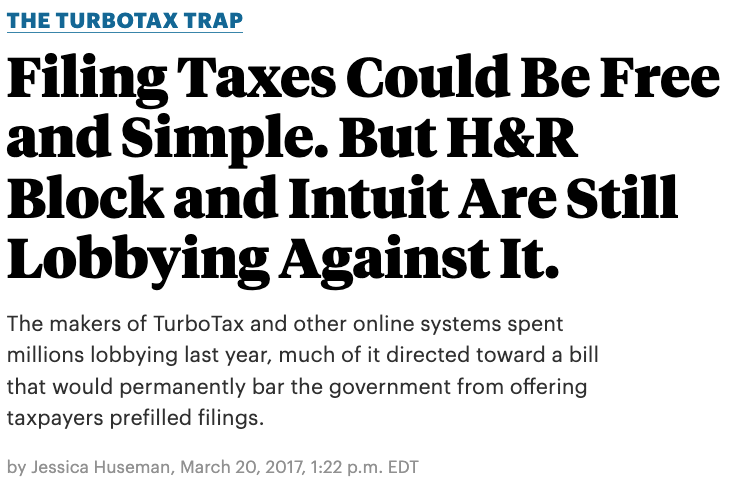
\includegraphics[width=0.9\linewidth]{Figures_Slides/Screenshot_News.png}} 

%     \vspace{1.5em} % space between first and second

%     \fbox{
\includegraphics[width=0.9\linewidth]{Figures_Slides/Article2.png}} 

%     \vspace{0.2em} % space between second and third

%     \fbox{
\includegraphics[width=0.9\linewidth]{Figures_Slides/Article_3_1.png}} 
% \end{center}
%   \end{column}
% \end{columns}
% \end{frame}


% \begin{frame}{Motivation: Tax Evasion}
% \begin{enumerate}
% \centering
%     \item \alert{Tax evasion} is a serious problem in many countries.
%     \vspace{1em}
% \end{enumerate}
%     %\begin{itemize}
%         %\item In the U.S. \$696B (15\%) taxes are not paid on time and \$606B (13\%) are never collected. \parencite{IRS_TaxGap_2022_Pub5869} 
%     %\end{itemize}
%     \begin{center}
%         \fbox{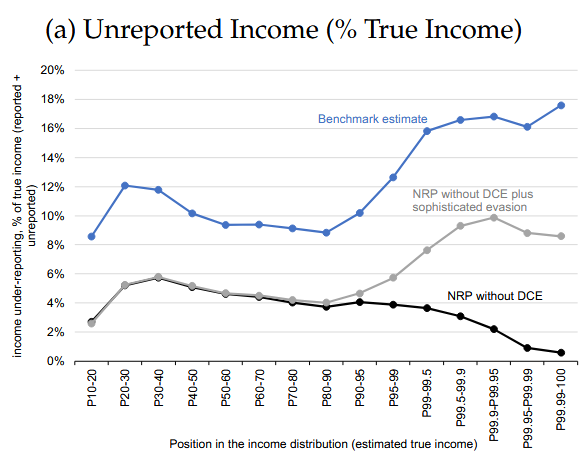
\includegraphics[width=0.45\linewidth]{Figures_Slides/Guyton.png}}
%     \end{center}
%     \vspace{-0.5em}
% \begin{enumerate}
% \centering
% \setcounter{enumi}{1}
%     \item Tax evasion is much \alert{more prevalent among the highest-income} earners. \parencite{guyton2021tax,alstadsaeter2019tax}
% \end{enumerate}
% \end{frame}



\begin{frame}
\frametitle{Information-Sharing (e.g., Third-Party Reporting)}
\begin{enumerate}
    \item Information exchange is \alert{highly effective to reduce tax evasion} \parencite{kleven2011unwilling,pomeranz2015no,slemrod2017does}
    \vspace{0.5em}
    \item The IRS needs information to \alert{prepopulate tax returns}.
\end{enumerate}
\vspace{2em}
Big potential: 
\vspace{0.5em}
\begin{itemize}
    \item In the U.S. \$696B (15\%) taxes are not paid on time and \$606B (13\%) are never collected \parencite{IRS_TaxGap_2022_Pub5869}.
    \vspace{0.5em}
    \item An average individual taxpayer has 13 hours and about \$250 tax filing costs \parencite{IRS2022}. This reflects a total cost of approximately \$100 billion per year. 
\end{itemize}
\end{frame}

\begin{frame}
\frametitle{Research Questions}
%Should the U.S. adopt more comprehensive information exchange? 
%\\
\vspace{1em}
%Why does the U.S. not yet offer (free tax software and) prepopulated tax returns?
\alert{What do people think} about comprehensive information exchange and \alert{how do they reason}?
\vspace{1em}
\begin{itemize}
    \item Focus on evasion considerations (revenue and fairness)?\\[0.2em]
    \item Focus on tax filing considerations?
    % \item Many other countries already do this.\\[0.2em]
    % \item Tax preparers in the US lobby against it.
\end{itemize}
% \vspace{1em}
% What do people think about such policies?
% \begin{itemize}
%     \item Do people support comprehensive information exchange and government provided tax filing services?  \\[0.2em]
%     \item What are people's reasons and considerations for their policy views?
%\end{itemize}
\end{frame}

% \begin{frame}
% \frametitle{What We Plan to Do}
% \begin{itemize}
%     \item We explore \alert{attitudes} and considerations \alert{towards information-sharing and tax filing service provision}.
%     \begin{itemize}
%         \item Towards more comprehensive third-party reporting and international automatic exchange of information. \\[0.2em]
%         \item Towards free tax software and/or prepopulated tax returns.
%     \end{itemize}
%     \vspace{1em} 
%     \item We leverages a \alert{large-scale survey to uncover considerations and beliefs} underlying these policy views.
%     \begin{itemize}
%         \item How, and why do they differ among respondents?
%     \end{itemize}
%     \vspace{1em} 
%     \item \alert{Experimental information} provision to establish \alert{causal} links between considerations and support for the policies.
% \end{itemize}
% \end{frame}

\begin{frame}{What We Plan to Do}
\begin{itemize}
\item Using a survey \alert{we explore peoples' attitudes and considerations towards information-sharing and free tax filing services.} 
\begin{itemize}
\item Third-party reporting and international exchange of information.
\item Free tax software and prepopulated tax returns.
\end{itemize}
\vspace{0.5em}
\item We include questions to \alert{uncover important drivers of policy views.}
\begin{itemize}
    \item Perceptions, beliefs and important considerations 
\end{itemize}
\vspace{0.5em}
\item To \alert{establish causal links} between reasoning and policy views, we randomize participants to different informational \alert{videos}.
\end{itemize}
\end{frame}


\begin{frame}{Measuring Policy Support}
\begin{columns}[T] % align columns at the top
  \begin{column}{0.45\textwidth} % left side for text
    \begin{itemize}
    \item Questions to uncover underlying considerations
    \begin{itemize}
        \item Knowledge
        \item Attitudes, perceptions, beliefs
        \item Reasoning
       % \item Policy support
    \end{itemize}
    \vspace{1em} 
    \item Provide \alert{policy-related information}
    \begin{itemize}
        \item Analyze how factors and considerations shape policy support
    \end{itemize}
    \end{itemize}
  \end{column}
  
  \begin{column}{0.45\textwidth} % right side for image
    \centering
    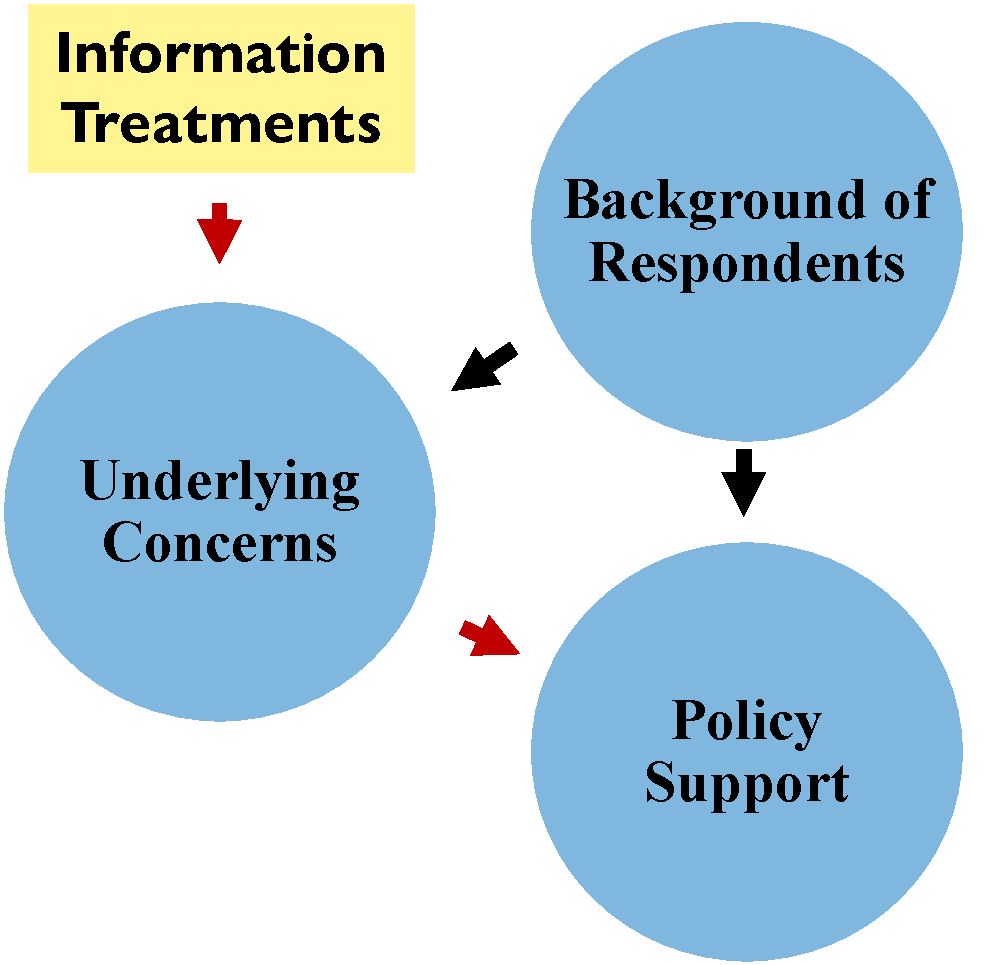
\includegraphics[width=\linewidth]{Figures_Slides/Estimation_Strategy.pdf}
  \end{column}
\end{columns}
\end{frame}

% \begin{frame}
% \frametitle{Related Literature}
% \begin{enumerate}
%     \item Measuring support for economic policies using survey experiments
% \begin{itemize}
% \scriptsize
%     \item Tax policy: {\tiny\textcite{stantcheva2021understanding}} \\[0.1em]
%     Tax simplicity and tax progressivity: {\tiny\textcite{tarroux2019value}} 
%     %\item Designing information provision experiments: {\footnotesize\textcite{haaland2023designing}}\\[0.2em]  
%     %Run surveys: {\footnotesize\textcite{stantcheva2023run}}.
% \end{itemize}
% \scriptsize
%     \item[$\Rightarrow$] \alert{Measuring support for information exchange and tax filing services.}
% \end{enumerate}
% \begin{enumerate}
% \setcounter{enumi}{1}
% \item Tax evasion, tax enforcement and information reporting
% \begin{itemize}
% \scriptsize
%     \item Third-party reporting: {\tiny \textcite{kleven2011unwilling}, \textcite{pomeranz2015no}, \textcite{kleven2016can}, \textcite{slemrod2017does}, \textcite{jensen2022employment}} \\[0.1em]
%     Automatic exchange of information: {\tiny \textcite{baselgia2023compliance}, \textcite{boas2024taxing}} \\[0.1em]
%     \item Distribution of tax evasion: {\tiny \textcite{johns2010distribution}, \textcite{alstadsaeter2019tax}, \textcite{guyton2021tax}}  
% \end{itemize}
% \scriptsize
% \item[$\Rightarrow$] \alert{How do these documented facts shape policy support for information exchange?}
% \vspace{0.2em} 
% \end{enumerate}
% \begin{enumerate}
% \setcounter{enumi}{2}
% \item Tax compliance costs and government's role to reduce them 
% \begin{itemize}
% \scriptsize
%     \item Tax filing costs: {\tiny\textcite{blumenthal1992compliance}, \textcite{benzarti2020taxing}}  \\[0.1em]
%     Non-filing: {\tiny\textcite{hauck2024optional}} \\[0.1em]
%     Tax complexity: {\tiny\textcite{benzarti2024rising}, \textcite{tarroux2019value}}  \\[0.1em]
%     \item Prepopulated tax returns: {\tiny\textcite{goodman2023automated}} \\[0.1em]
% \end{itemize}
% \scriptsize
% \item[$\Rightarrow$] \alert{Analyse support for prepopulated tax returns and tax software (and its drivers).} 
% \item[$\Rightarrow$] \alert{Explore the relation of support for tax filing services with support for information sharing.}
% \end{enumerate}
% \end{frame}


\section{Survey and Sample}

\begin{frame}{Recruitment and Screening}
\begin{columns}[T] % align columns at the top
  \begin{column}{0.45\textwidth} % left side for text
    \begin{itemize}
    \item U.S. residents aged 18 to 69 recruited through a commercial survey company (e.g. Prolific / Bilendi)
    \vspace{1em} 
    \item \alert{Quota representativity} 
    \begin{itemize}
        \item Dimensions gender, age, region and education
    \end{itemize}
%    \vspace{1em} 
%    \item \alert{Avoid selection}
%    \begin{itemize}
%        \item Recruit without revealing topic / identity
%    \end{itemize}
    \vspace{1em} 
    \item Embedded attention checks for high-quality responses. 
    \end{itemize}
  \end{column}
  
  \begin{column}{0.45\textwidth} % right side for image
    \centering
    \vspace{-2em}
    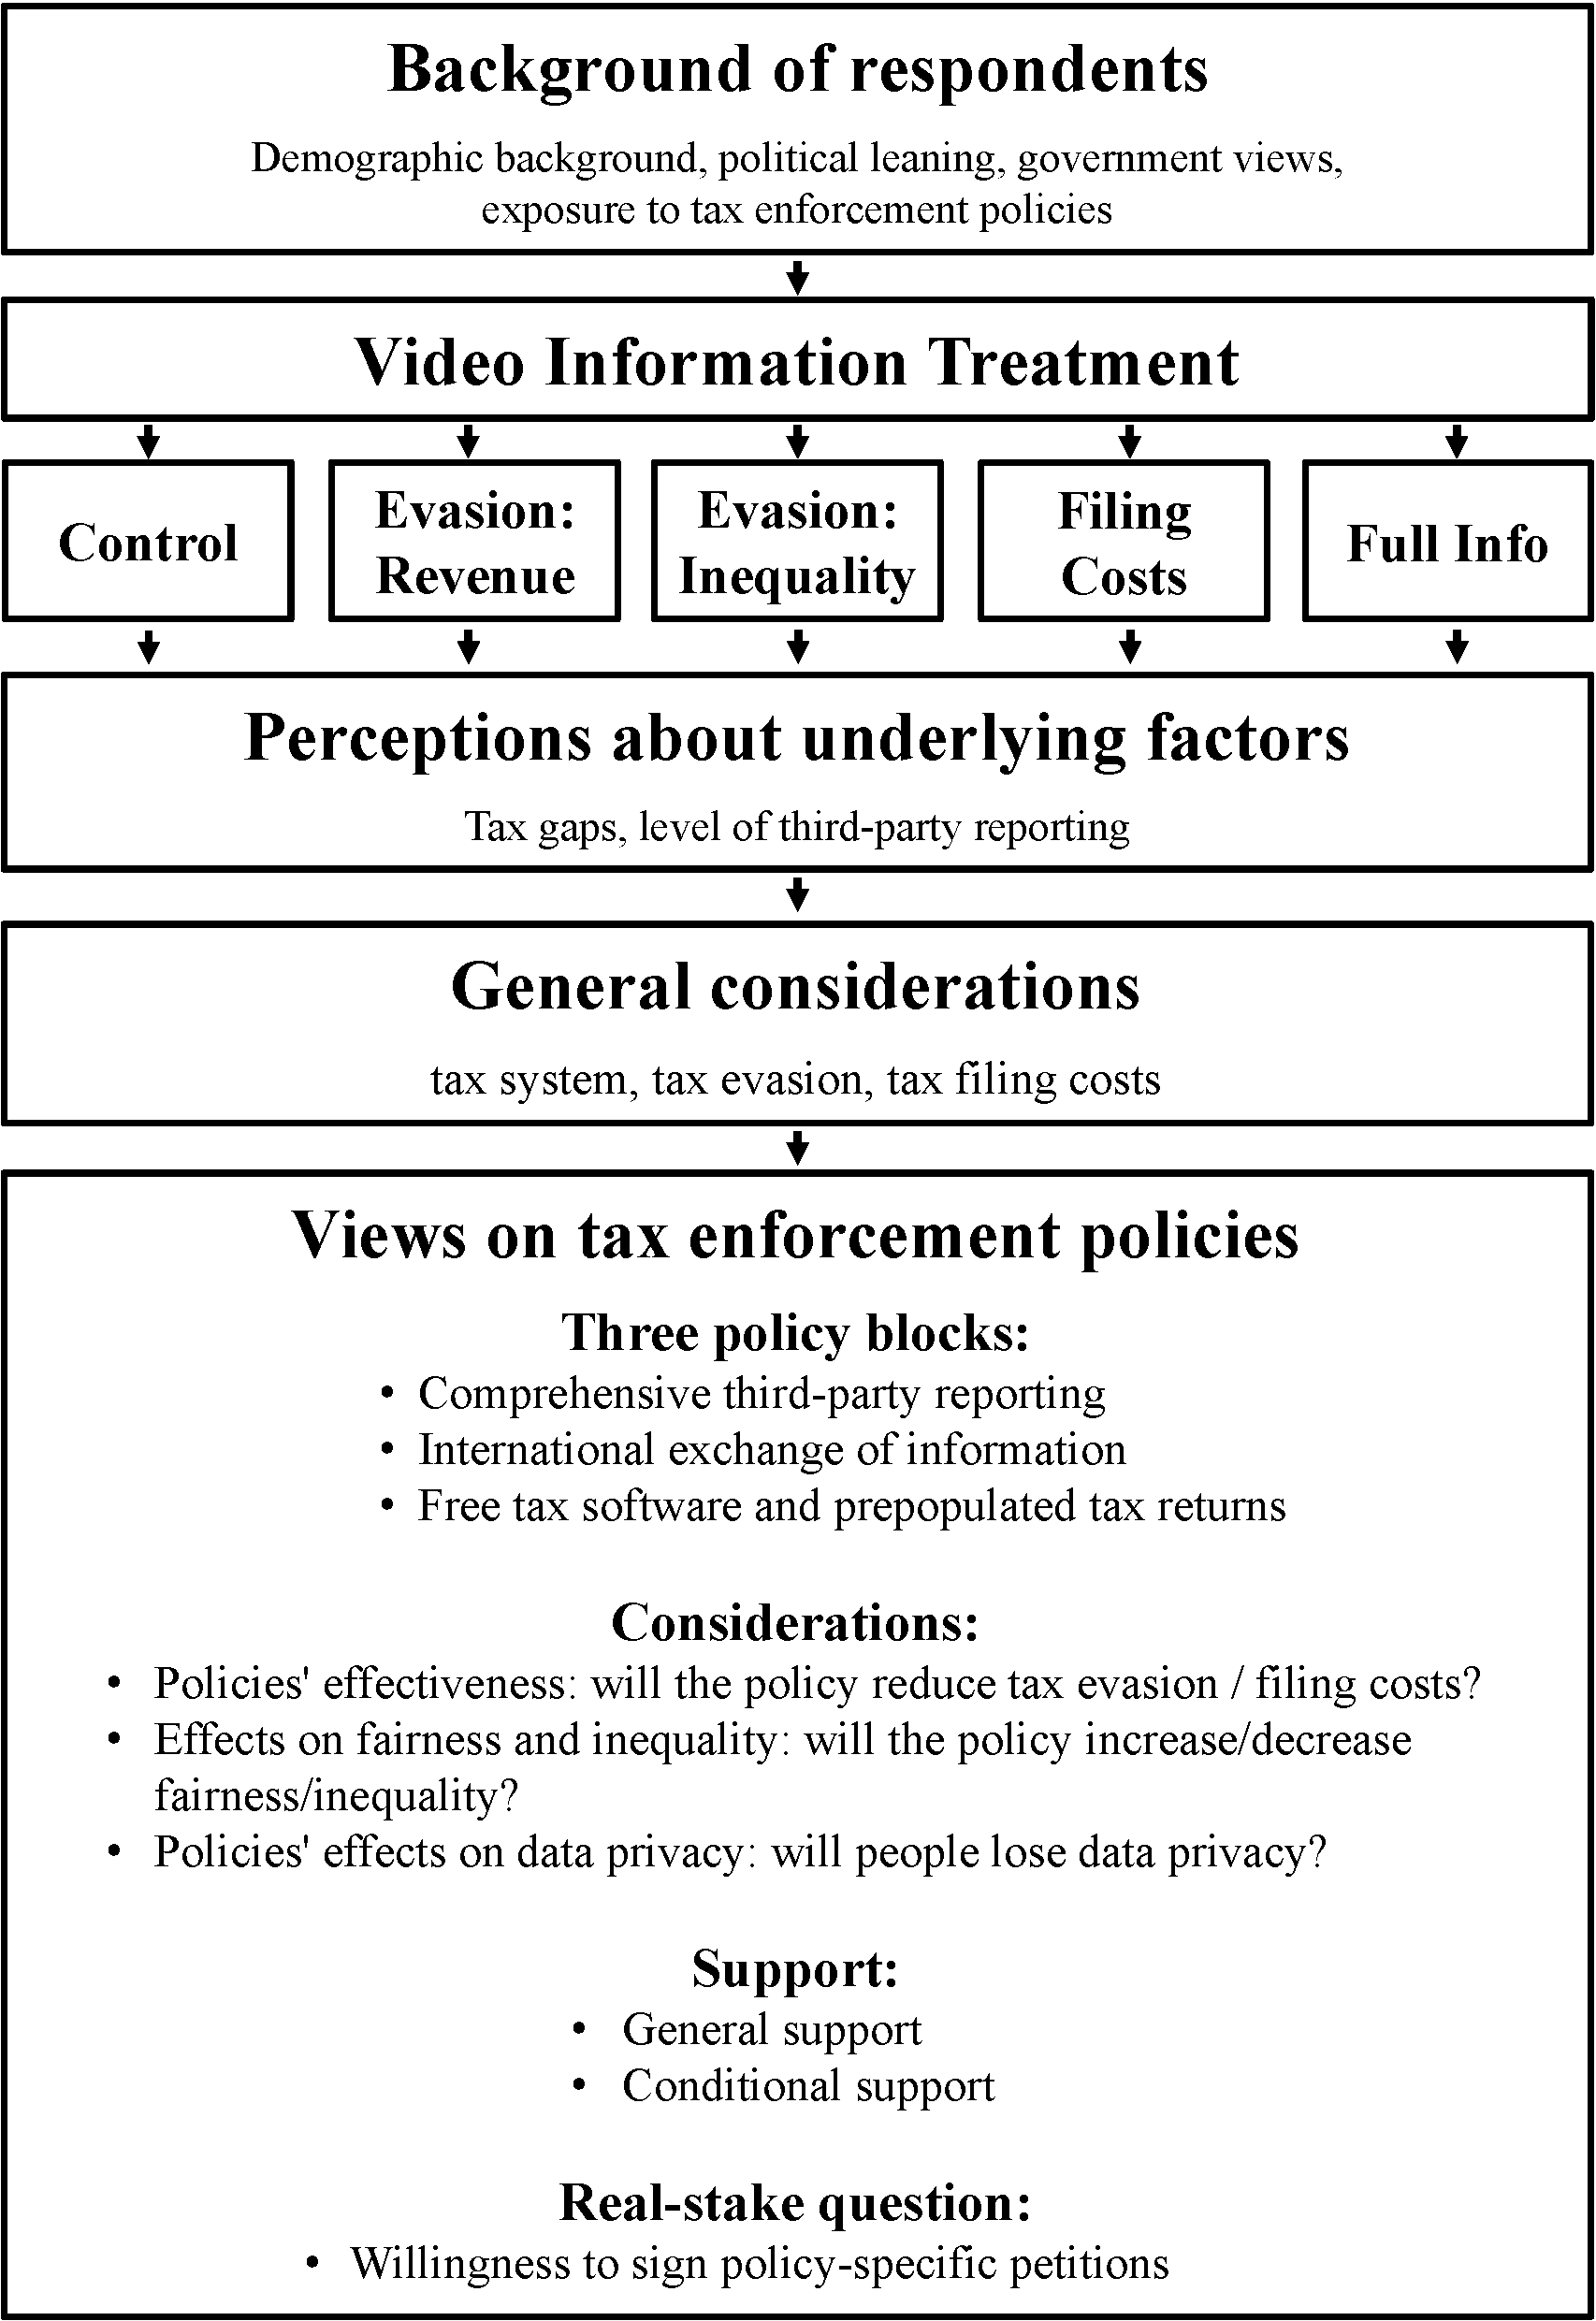
\includegraphics[width=1.05\linewidth]{Figures_Slides/Survey_Overview_Blank.pdf}
  \end{column}
\end{columns}
\end{frame}

% \begin{frame}[label=Personal_Exposure]{Background of Respondents}
% \begin{columns}[T] % align columns at the top
%   \begin{column}{0.45\textwidth} % left side for text
%     \begin{itemize}
%     \item Demographic background %(age, education, region, income, ethnicity, household composition) 
%     \vspace{0.5em} 
%     \item Political leaning
%     \begin{itemize}
%         \item Voting behavior
%         \item Liberal/conservative
%         \item Political affiliation
%     \end{itemize}
%     \vspace{0.5em} 
%     \item Government views
%     \begin{itemize}
%         \item Trust
%         \item Desired involvement
%         \item Quality of services
%     \end{itemize}
%     \vspace{0.5em} 
%     \item \alert{Exposure} to taxes \hyperlink{Personal_Exposure_Appendix}{\beamergotobutton{A: PE}}
%     \begin{itemize}
%         \item Tax filing
%         \item Filing mistakes and evasion
%     \end{itemize}
%     \end{itemize}
%   \end{column}
  
%   \begin{column}{0.45\textwidth} % right side for image
%     \centering
%      \vspace{-2em}
%     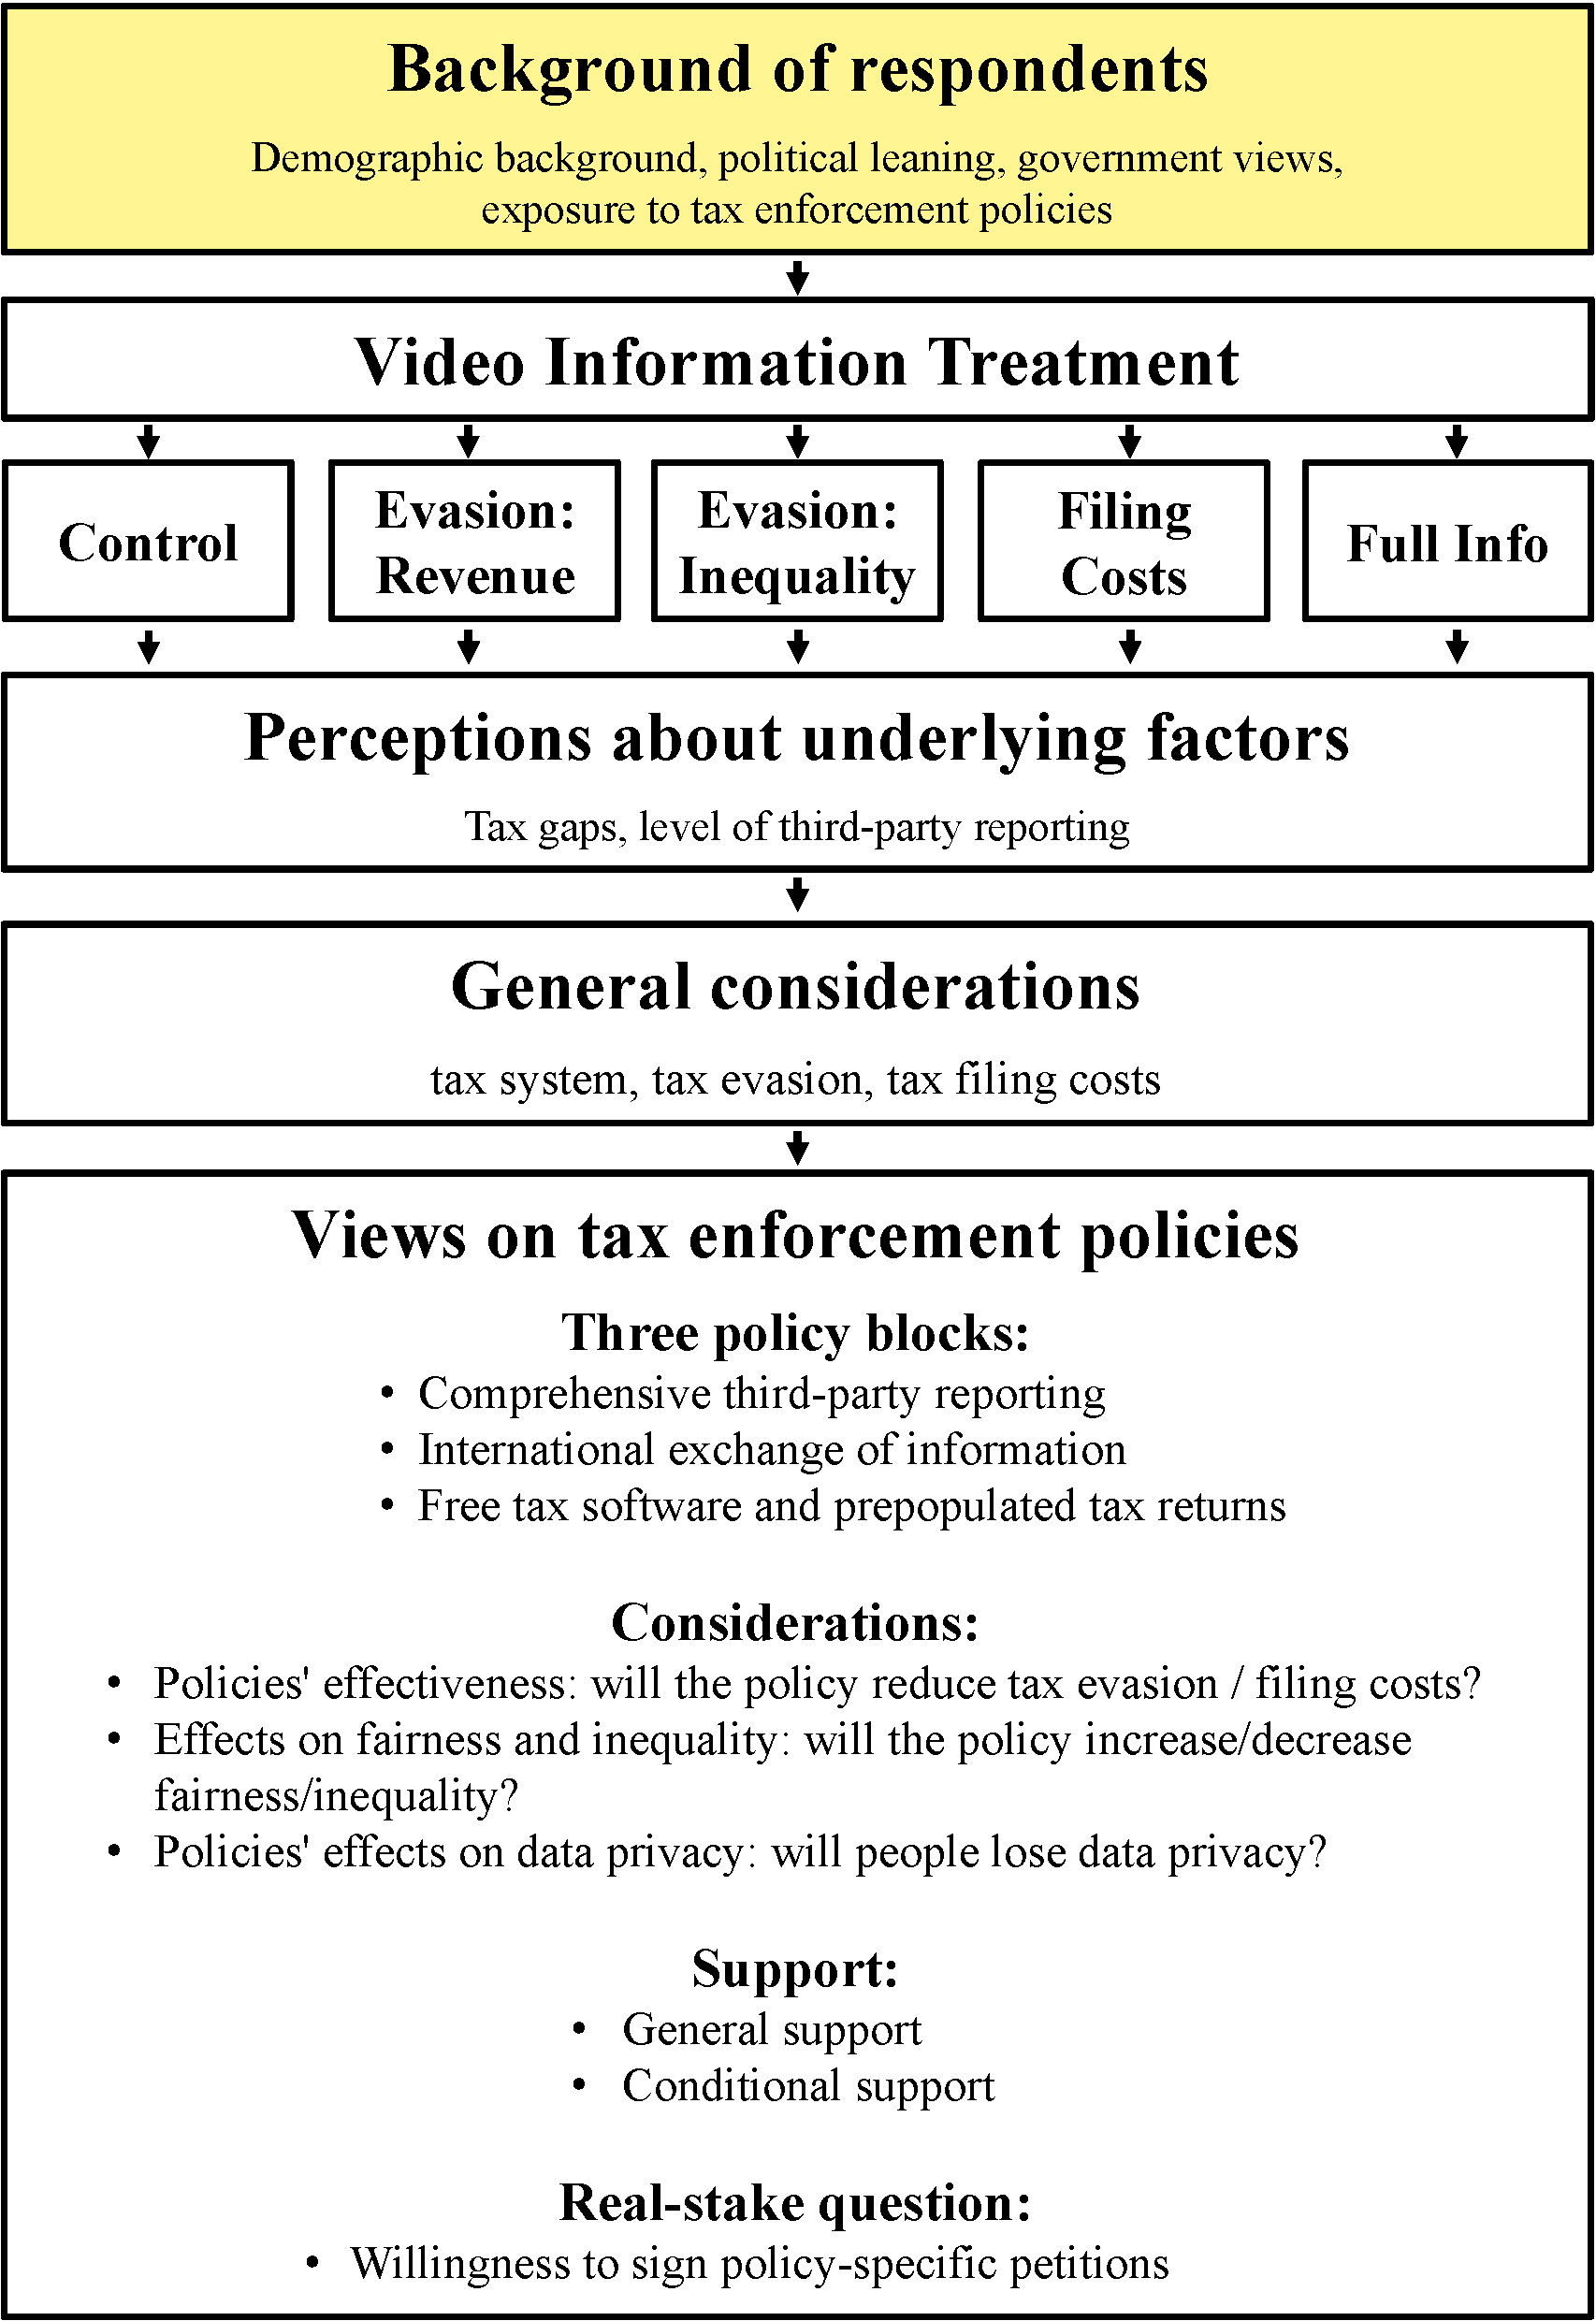
\includegraphics[width=1.05\linewidth]{Figures_Slides/Survey_Overview_Background.pdf}
%   \end{column}
% \end{columns}
% \end{frame}

%\begin{frame}{Video Information Treatments}
%\begin{columns}[T] % align columns at the top
%  \begin{column}{0.45\textwidth} % left side for text
%    \begin{itemize}
%    \vspace{1em} 
%    \item Educational \alert{information videos}
%    \begin{itemize}
%        \item Audio
%        \item Subtitles
%        \item Animated
%    \end{itemize}
%    \vspace{1.5em} 
%    \item Close \alert{link to important underlying concerns} 
%    \begin{itemize}
%        \item Tax evasion \& revenue
%        \item Fairness \& inequality
%        \item Tax filing costs
%    \end{itemize}
%    \end{itemize}
%  \end{column}
%  
%  \begin{column}{0.45\textwidth} % right side for image
%    \centering
%     \vspace{-2em}     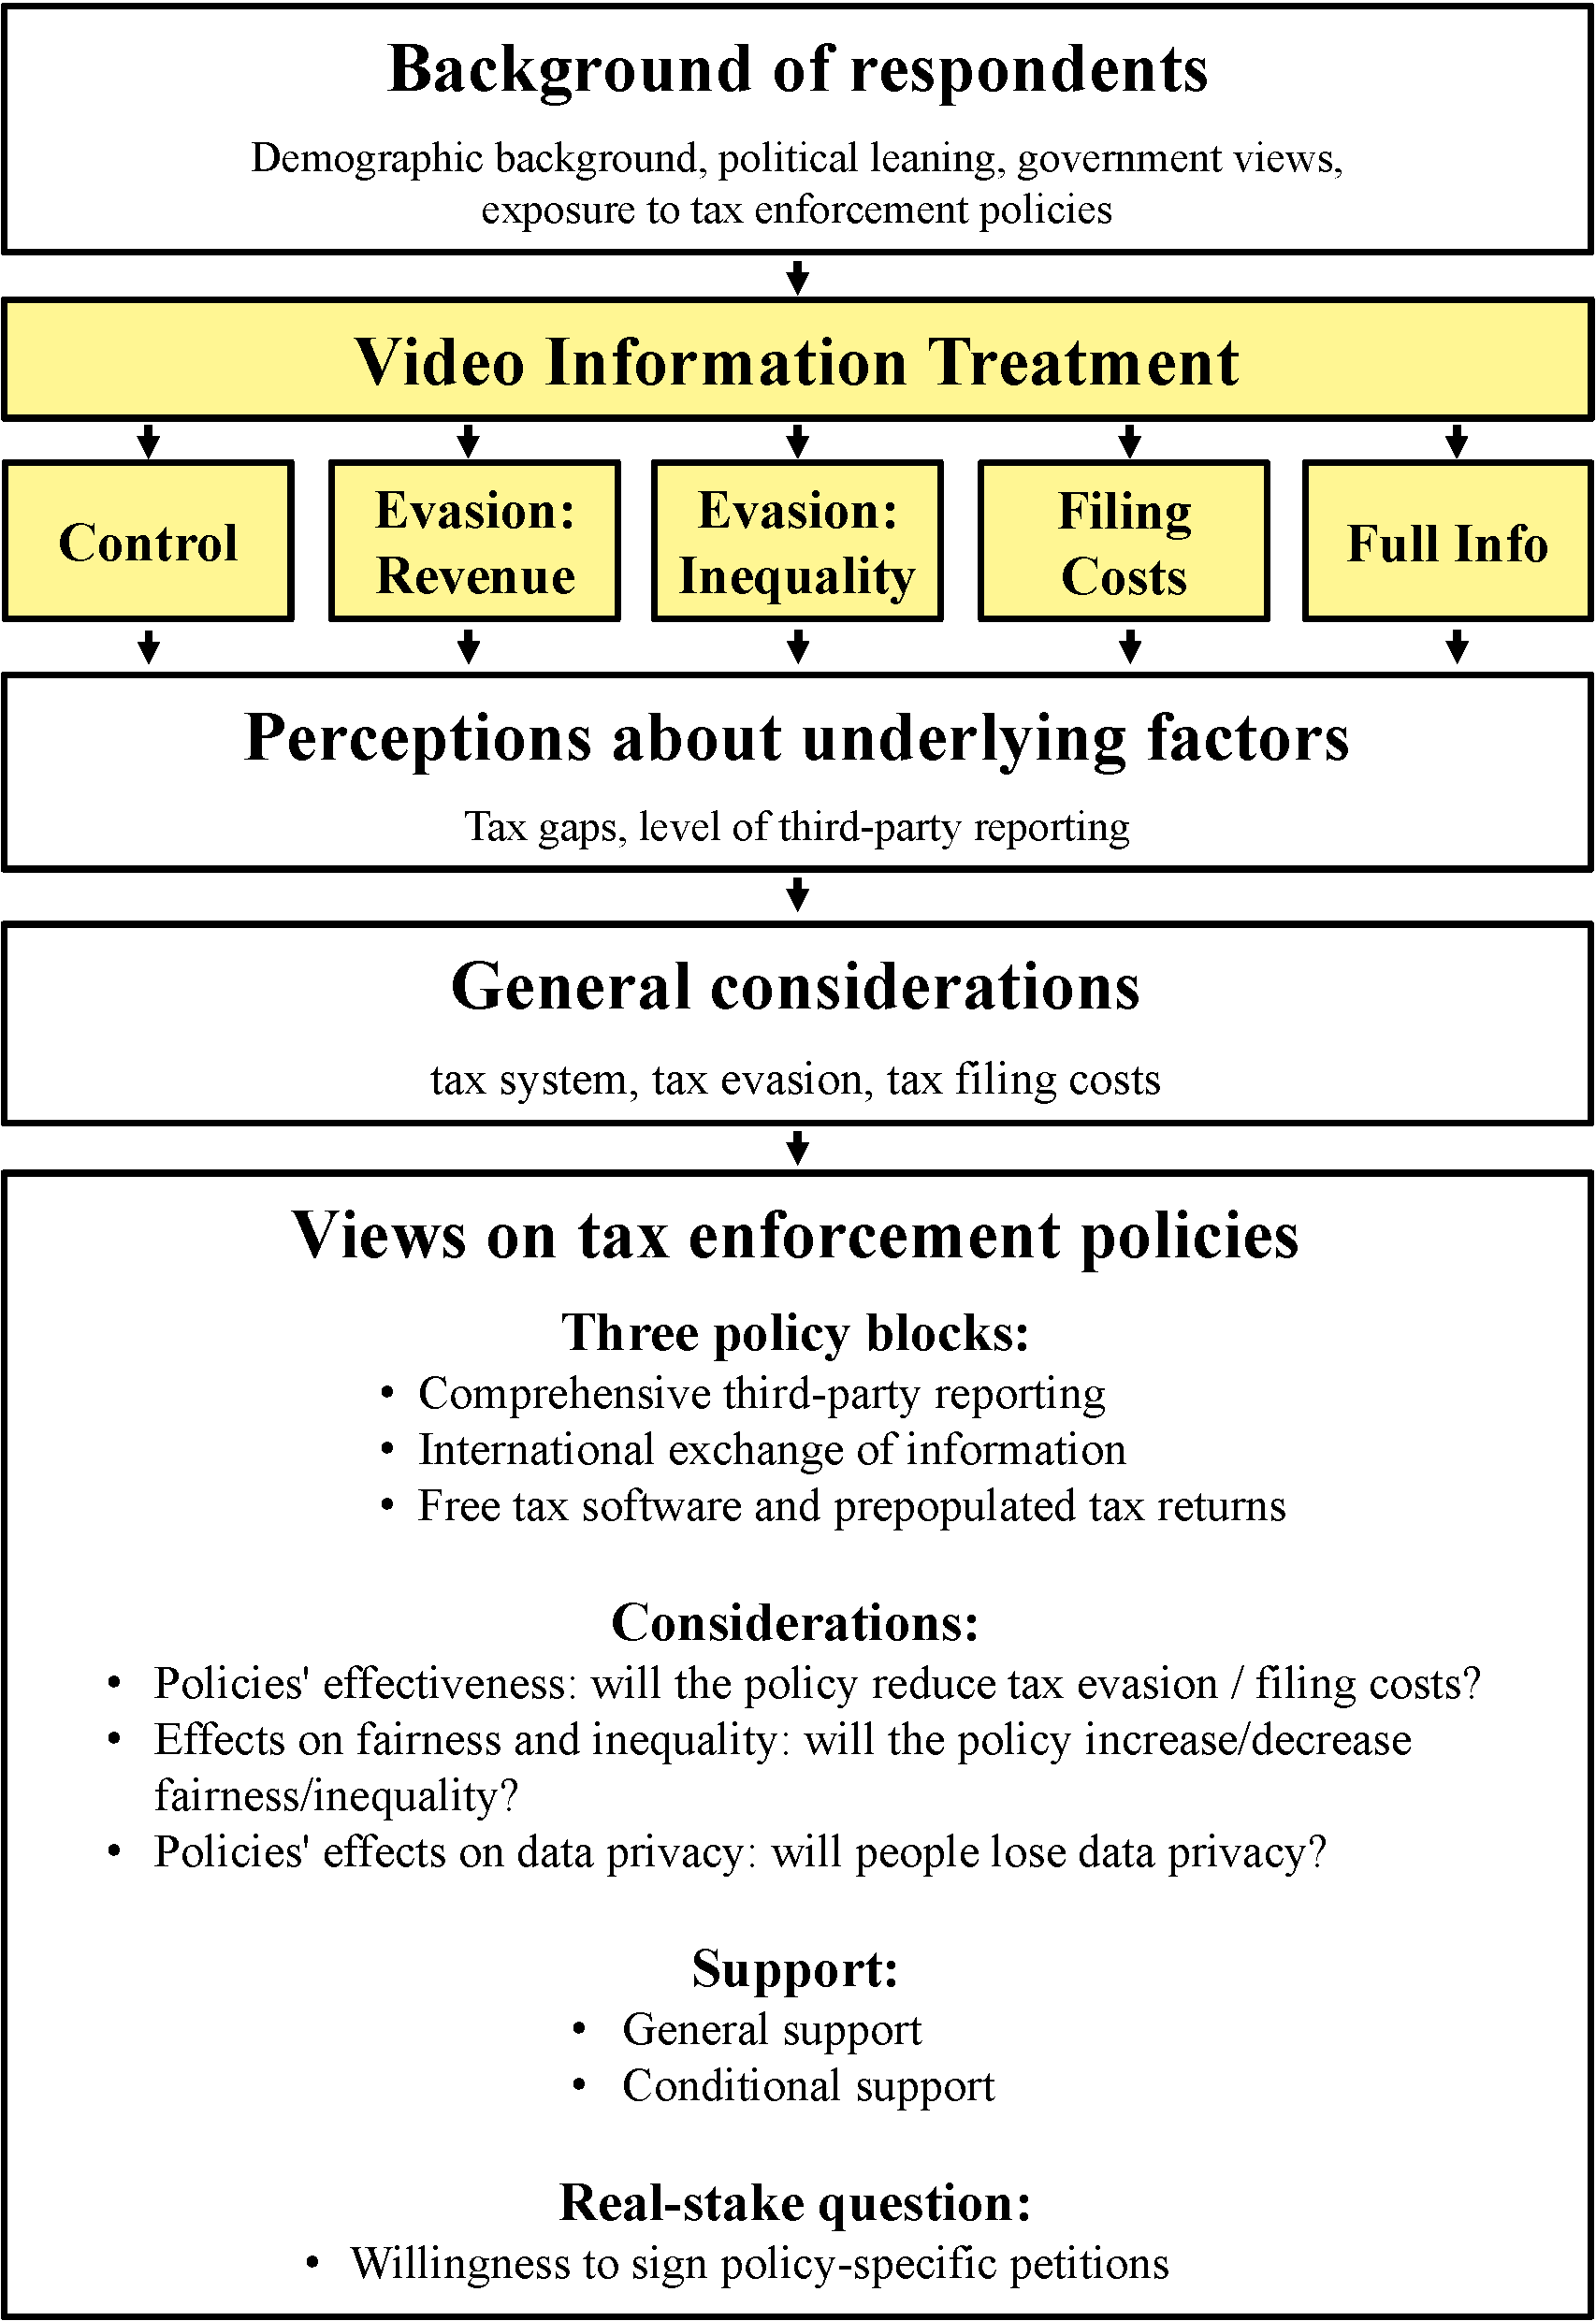
\includegraphics[width=1.05\linewidth]{Figures_Slides/Survey_Overview_Treatments.pdf}
%  \end{column}
%\end{columns}
%\end{frame}

% \begin{frame}{Video Information Treatments}
% \begin{columns}[T] % align columns at the top
%   \begin{column}{0.45\textwidth} % left side for text
%     \begin{itemize}
%     \vspace{1em} 
%     \item Educational \alert{information videos}
%     \begin{itemize}
%         \item Audio
%         \item Subtitles
%         \item Animated
%     \end{itemize}
%     \vspace{1.5em} 
%     \item Close \alert{link to important underlying concerns} 
%     \begin{itemize}
%         \item Tax evasion \& revenue
%         \item Fairness \& inequality
%         \item Tax filing costs
%     \end{itemize}
%     \end{itemize}
%   \end{column}
  
%   \begin{column}{0.45\textwidth} % right side for image
%     %\vspace{0.3cm}
%     \centering
%     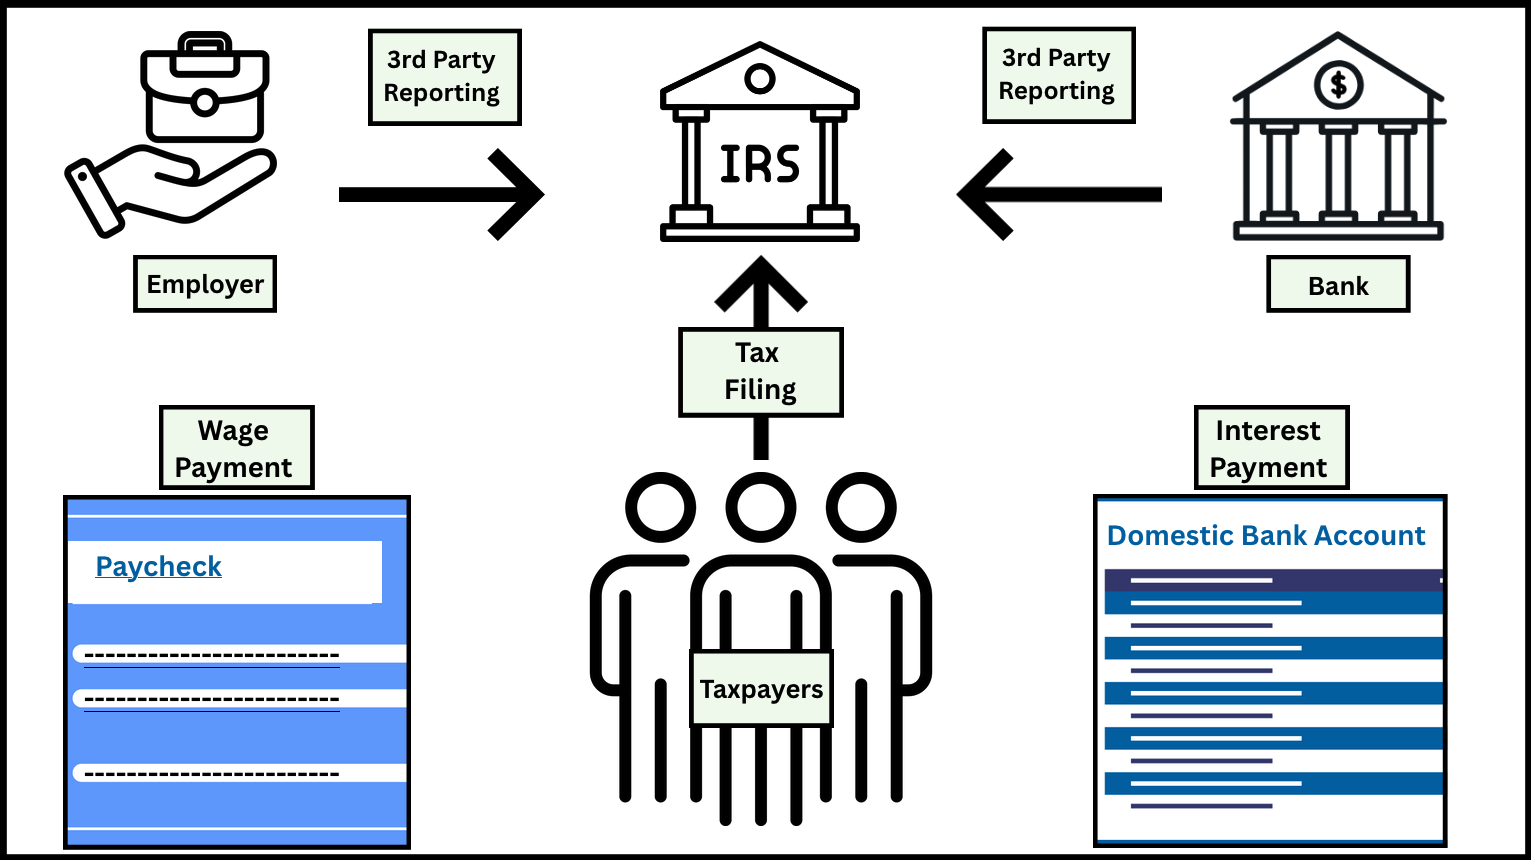
\includegraphics[width=0.95\linewidth]{Figures_Slides/Screenshot_3.png}\\[0.5cm]
%     %\vspace*{1cm}
%     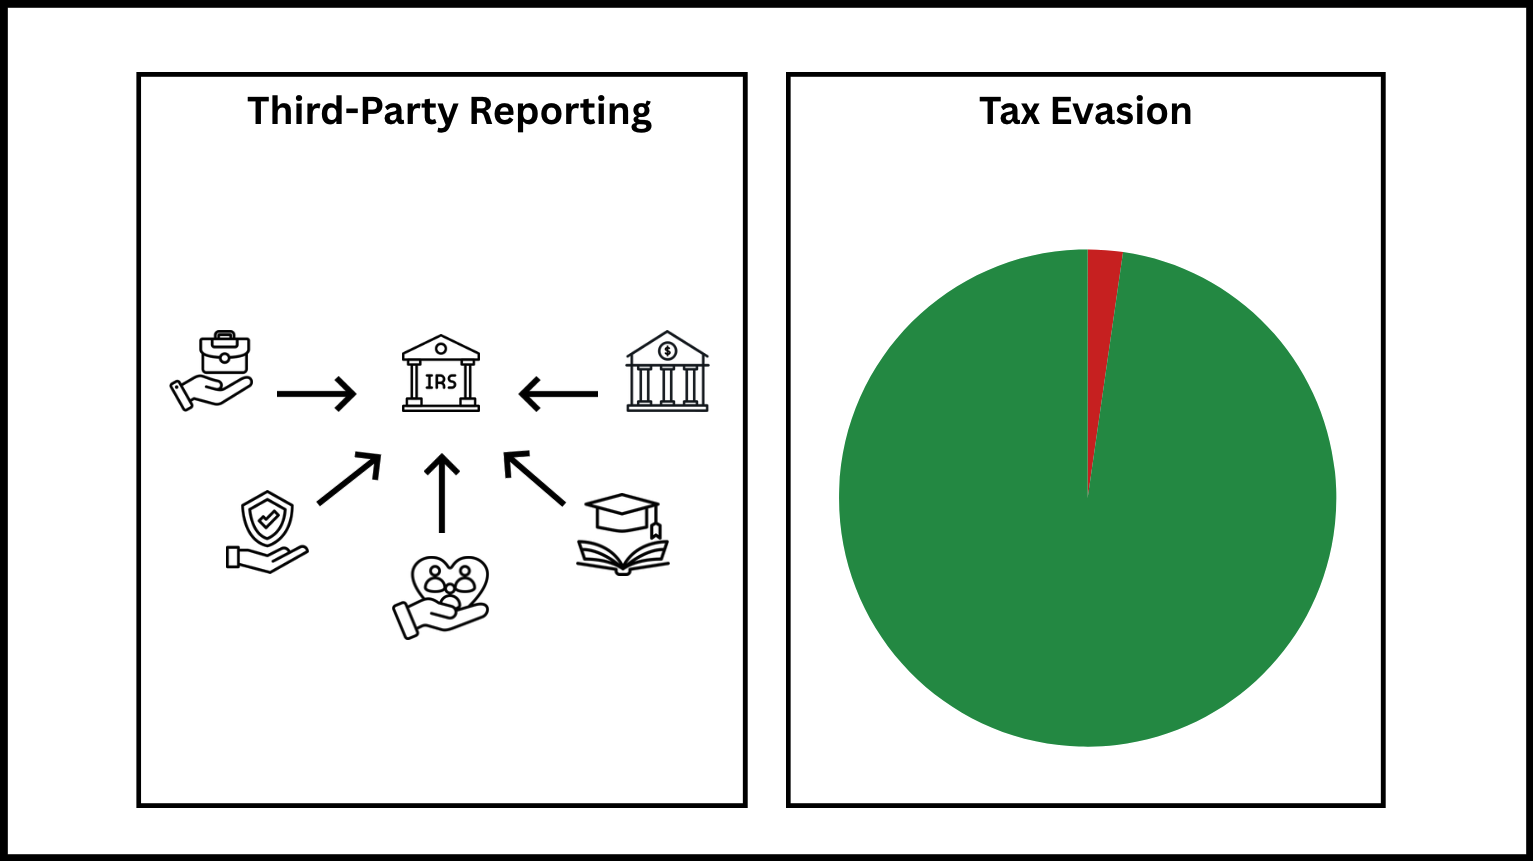
\includegraphics[width=0.95\linewidth]{Figures_Slides/Screenshot_2.png}
%   \end{column}
% \end{columns}
% \end{frame}

\begin{frame}
  \centering
  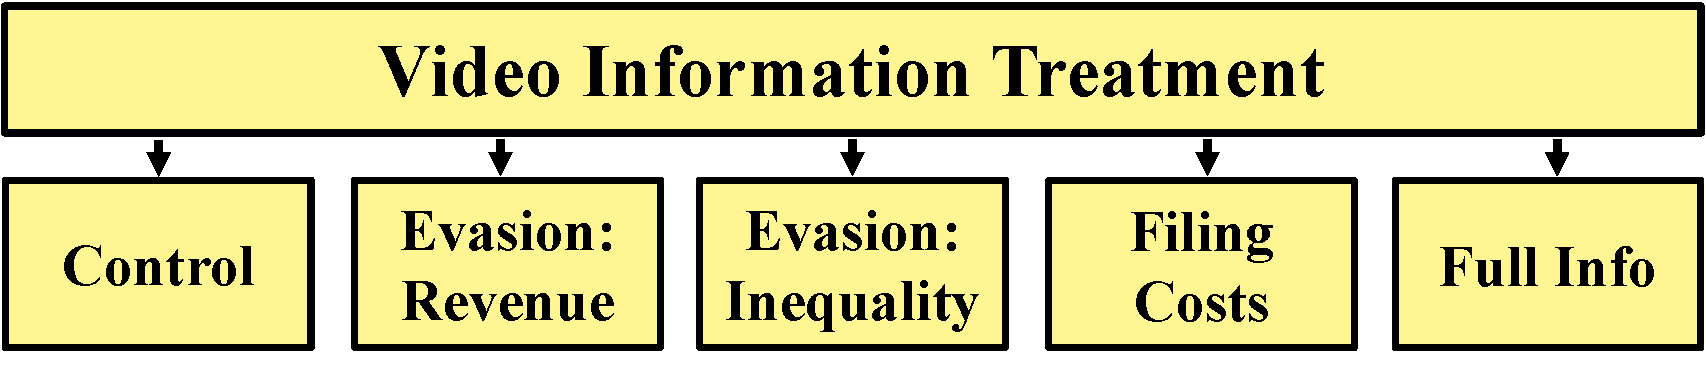
\includegraphics[width=0.7\textwidth]{Figures_Slides/Survey_Overview_Treatments_Focus.pdf}

  \vspace{1cm}
\centering
{\scriptsize
\begin{tabularx}{\textwidth}{*{3}{>{\centering\arraybackslash}X}}
  \textbf{Evasion: Revenue} & \textbf{Evasion: Inequality} & \textbf{Filing Costs} \\[-0.5em]
  \begin{itemize}\item \alert{Extent} of tax evasion\end{itemize} &
  \begin{itemize}\item \alert{Distribution} of tax evasion\end{itemize} &
  \begin{itemize}\item \alert{Filing costs} and tax software\end{itemize} \\[-2em]
  \begin{itemize}\item Third-party reporting \& AEoI \alert{reduces tax evasion}\end{itemize} &
  \begin{itemize}\item Third-party reporting \& AEoI \alert{reduces tax evasion}\end{itemize} &
  \begin{itemize}\item Third-party reporting is \alert{important for prepopulated returns}\end{itemize} \\[-2em]
  \begin{itemize}\item[$\Rightarrow$] Economic considerations\end{itemize} &
  \begin{itemize}\item[$\Rightarrow$] Inequality \& fairness considerations\end{itemize} &
  \begin{itemize}\item[$\Rightarrow$] Filing considerations\end{itemize} \\
\end{tabularx}
}
\centering
{\scriptsize
\begin{tabularx}{0.7\textwidth}{*{2}{>{\centering\arraybackslash}X}}
  \textbf{Control} & \textbf{Full Info} \\[-0.5em]
  \begin{itemize}\item No information \end{itemize} &
  \begin{itemize}\item Summary of all three treatments \end{itemize} \\[-2em]
\end{tabularx}
}%\hyperlink{thanks}{\beamergotobutton{Finish}}
\end{frame}

% \begin{frame}{Video Information Treatment:\\ Challenges}
% \begin{columns}[T] % align columns at the top
%   \begin{column}{0.45\textwidth} % left side for text
%     \begin{itemize}
%     \item Difficult to isolate data privacy concerns
%     \begin{itemize}
%         \item[$\Rightarrow$] Questions included to measure and control for them.  
%     \end{itemize}
%     \vspace{0.5em} 
%     \item Differing video lengths 
%     \begin{itemize}
%         \item[$\Rightarrow$] Full info treatment as "highlights" video to reduce differences in attrition
%     \end{itemize}
%     \vspace{0.5em} 
%     \item Non-lab setting 
%     \begin{itemize}
%         \item[$\Rightarrow$] Embedded attention checks
%     \end{itemize}
%     \end{itemize}
%   \end{column}
%   \begin{column}{0.45\textwidth} % right side for image
%     \centering
%      \vspace{-4em}     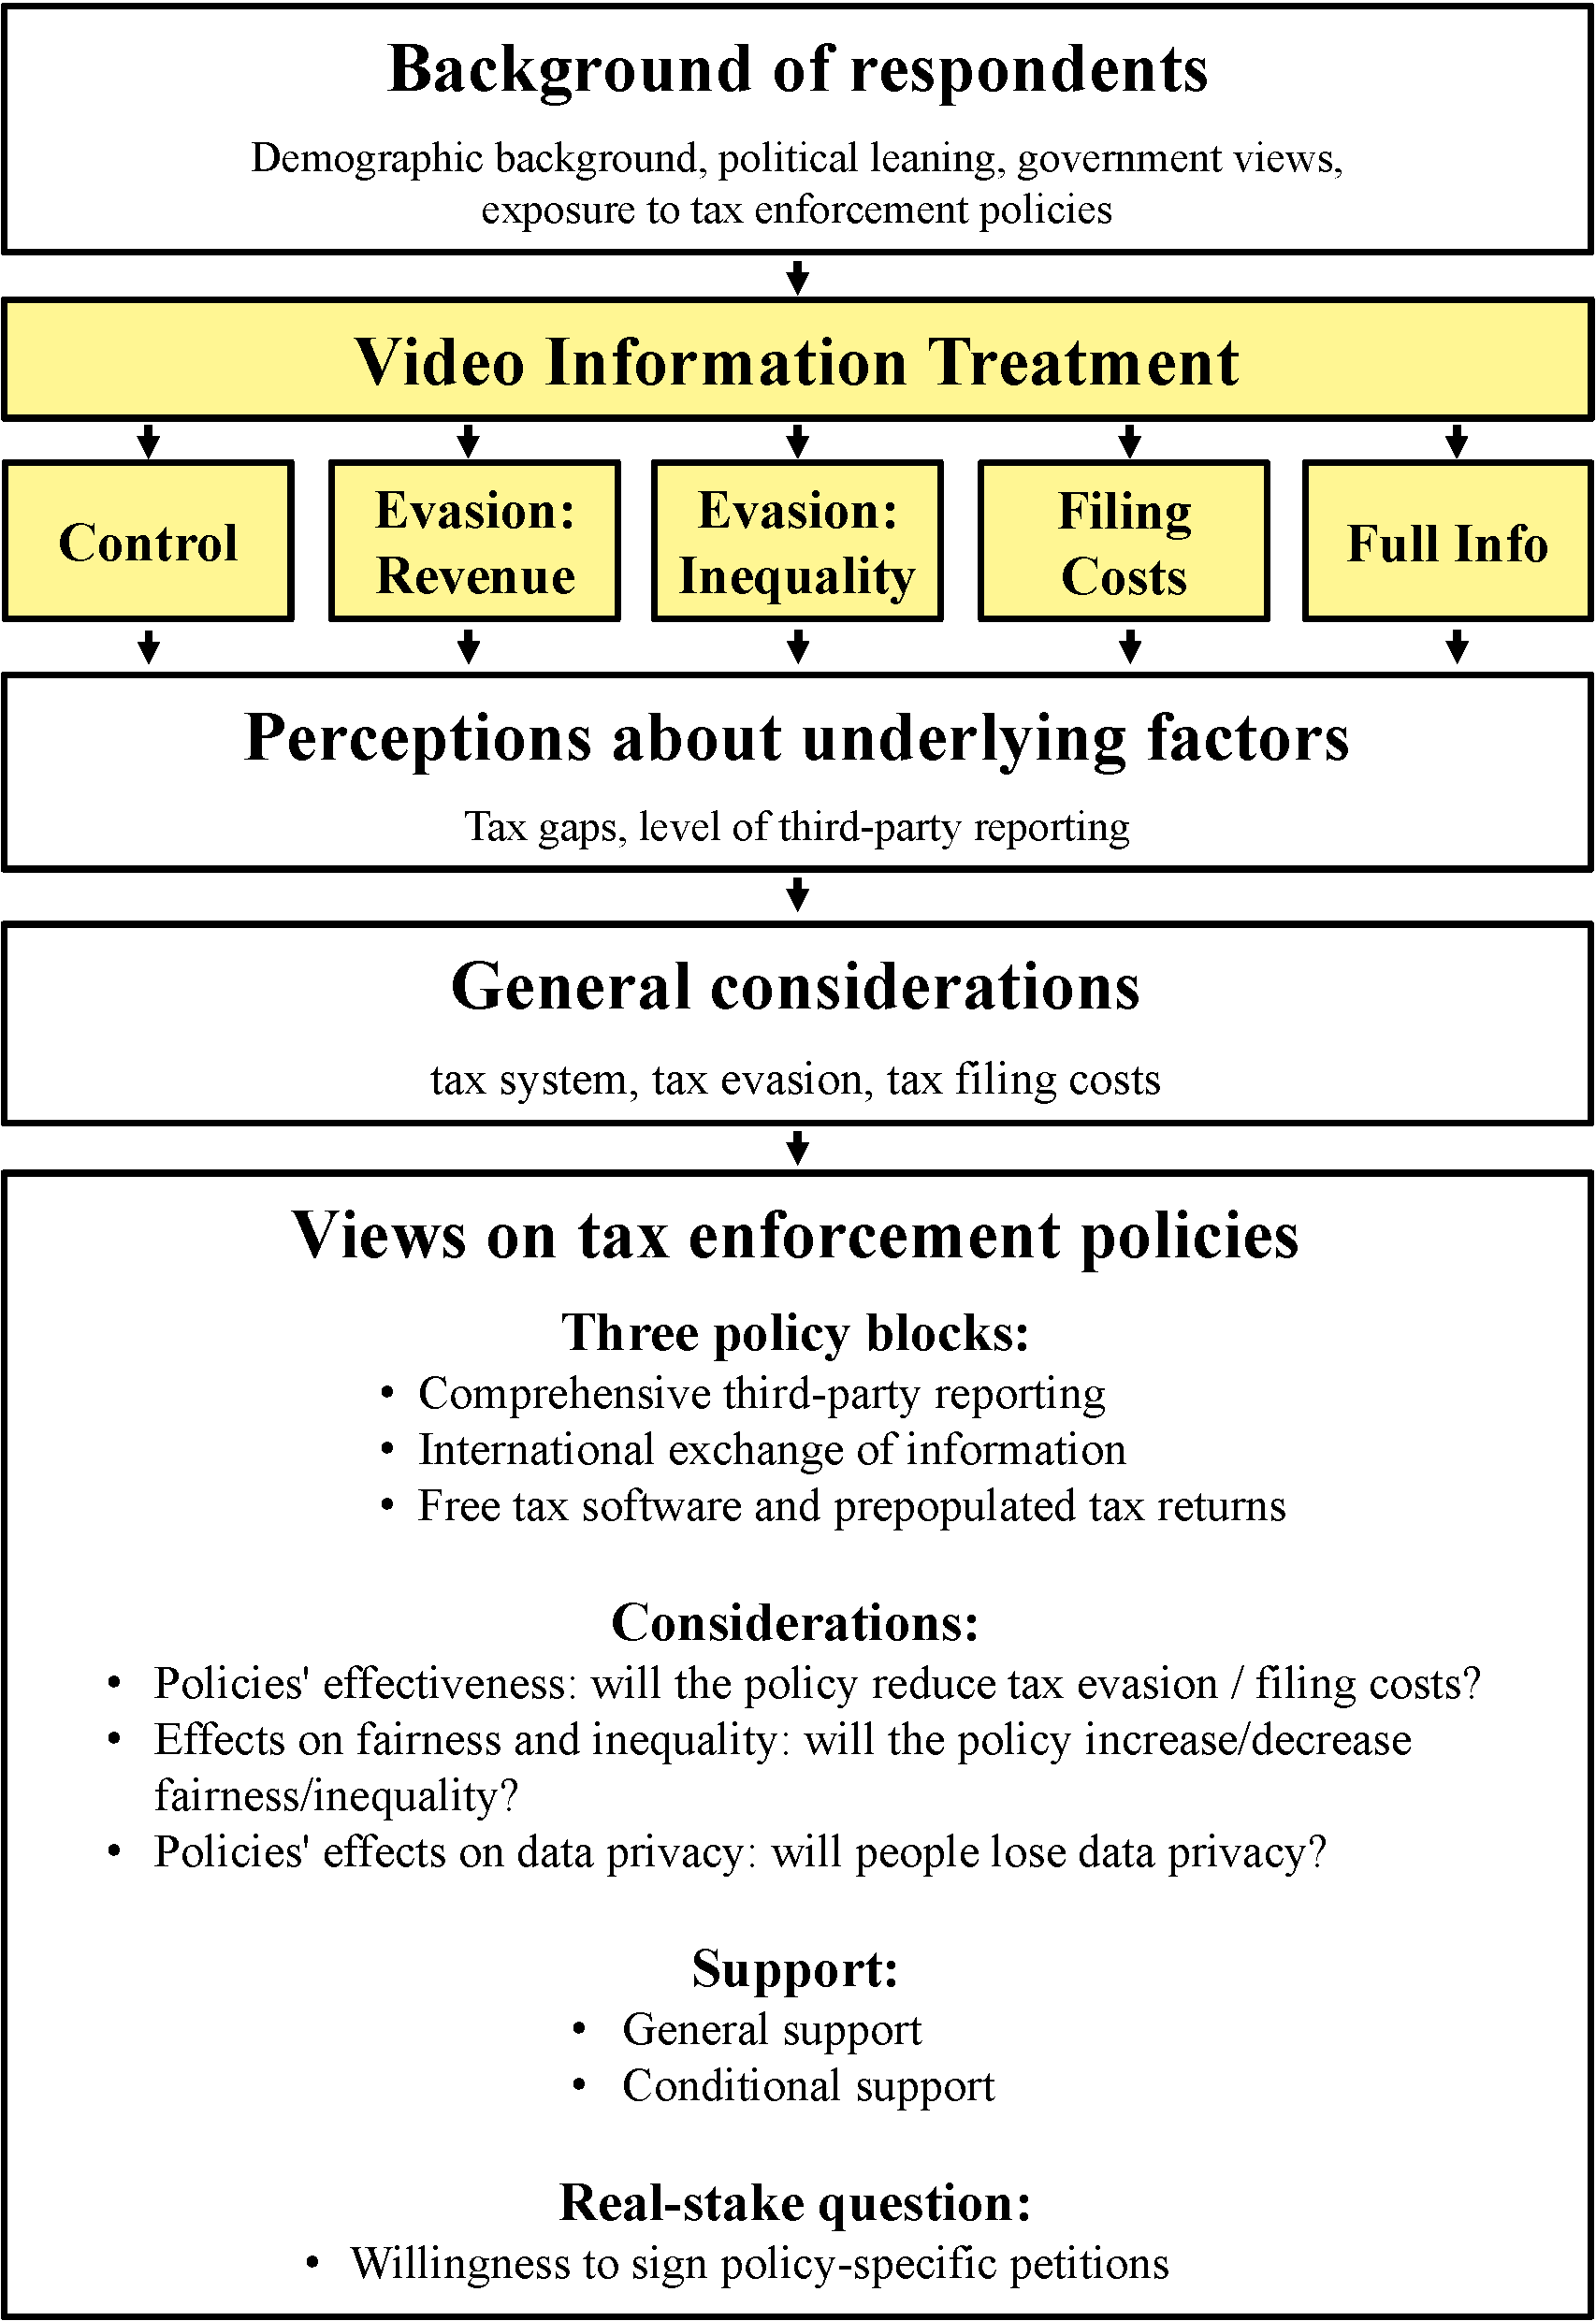
\includegraphics[width=1.05\linewidth]{Figures_Slides/Survey_Overview_Treatments.pdf}
%   \end{column}
% \end{columns}
% \end{frame}

% \begin{frame}[label=Prior_Perceptions]{Perceptions about Underlying \\ Factors}
% \begin{columns}[T] % align columns at the top
%   \begin{column}{0.45\textwidth} % left side for text
%     \begin{itemize}
%     \item Perceptions about tax gaps \hyperlink{Prior_Perceptions_Appendix}{\beamergotobutton{A: TG}}
%     \begin{itemize}
%         \item Overall tax gap 
%         \item Distribution of tax evasion across groups 
%     \end{itemize}
%     \vspace{0.5em} 
%     \item Perceptions about tax authorities' access to data
%     \vspace{2em} 
%     \item[$\Rightarrow$] Understand whether respondents update perceptions. 
%     \end{itemize}
%   \end{column}
  
%   \begin{column}{0.45\textwidth} % right side for image
%     \centering
%      \vspace{-4em}
%     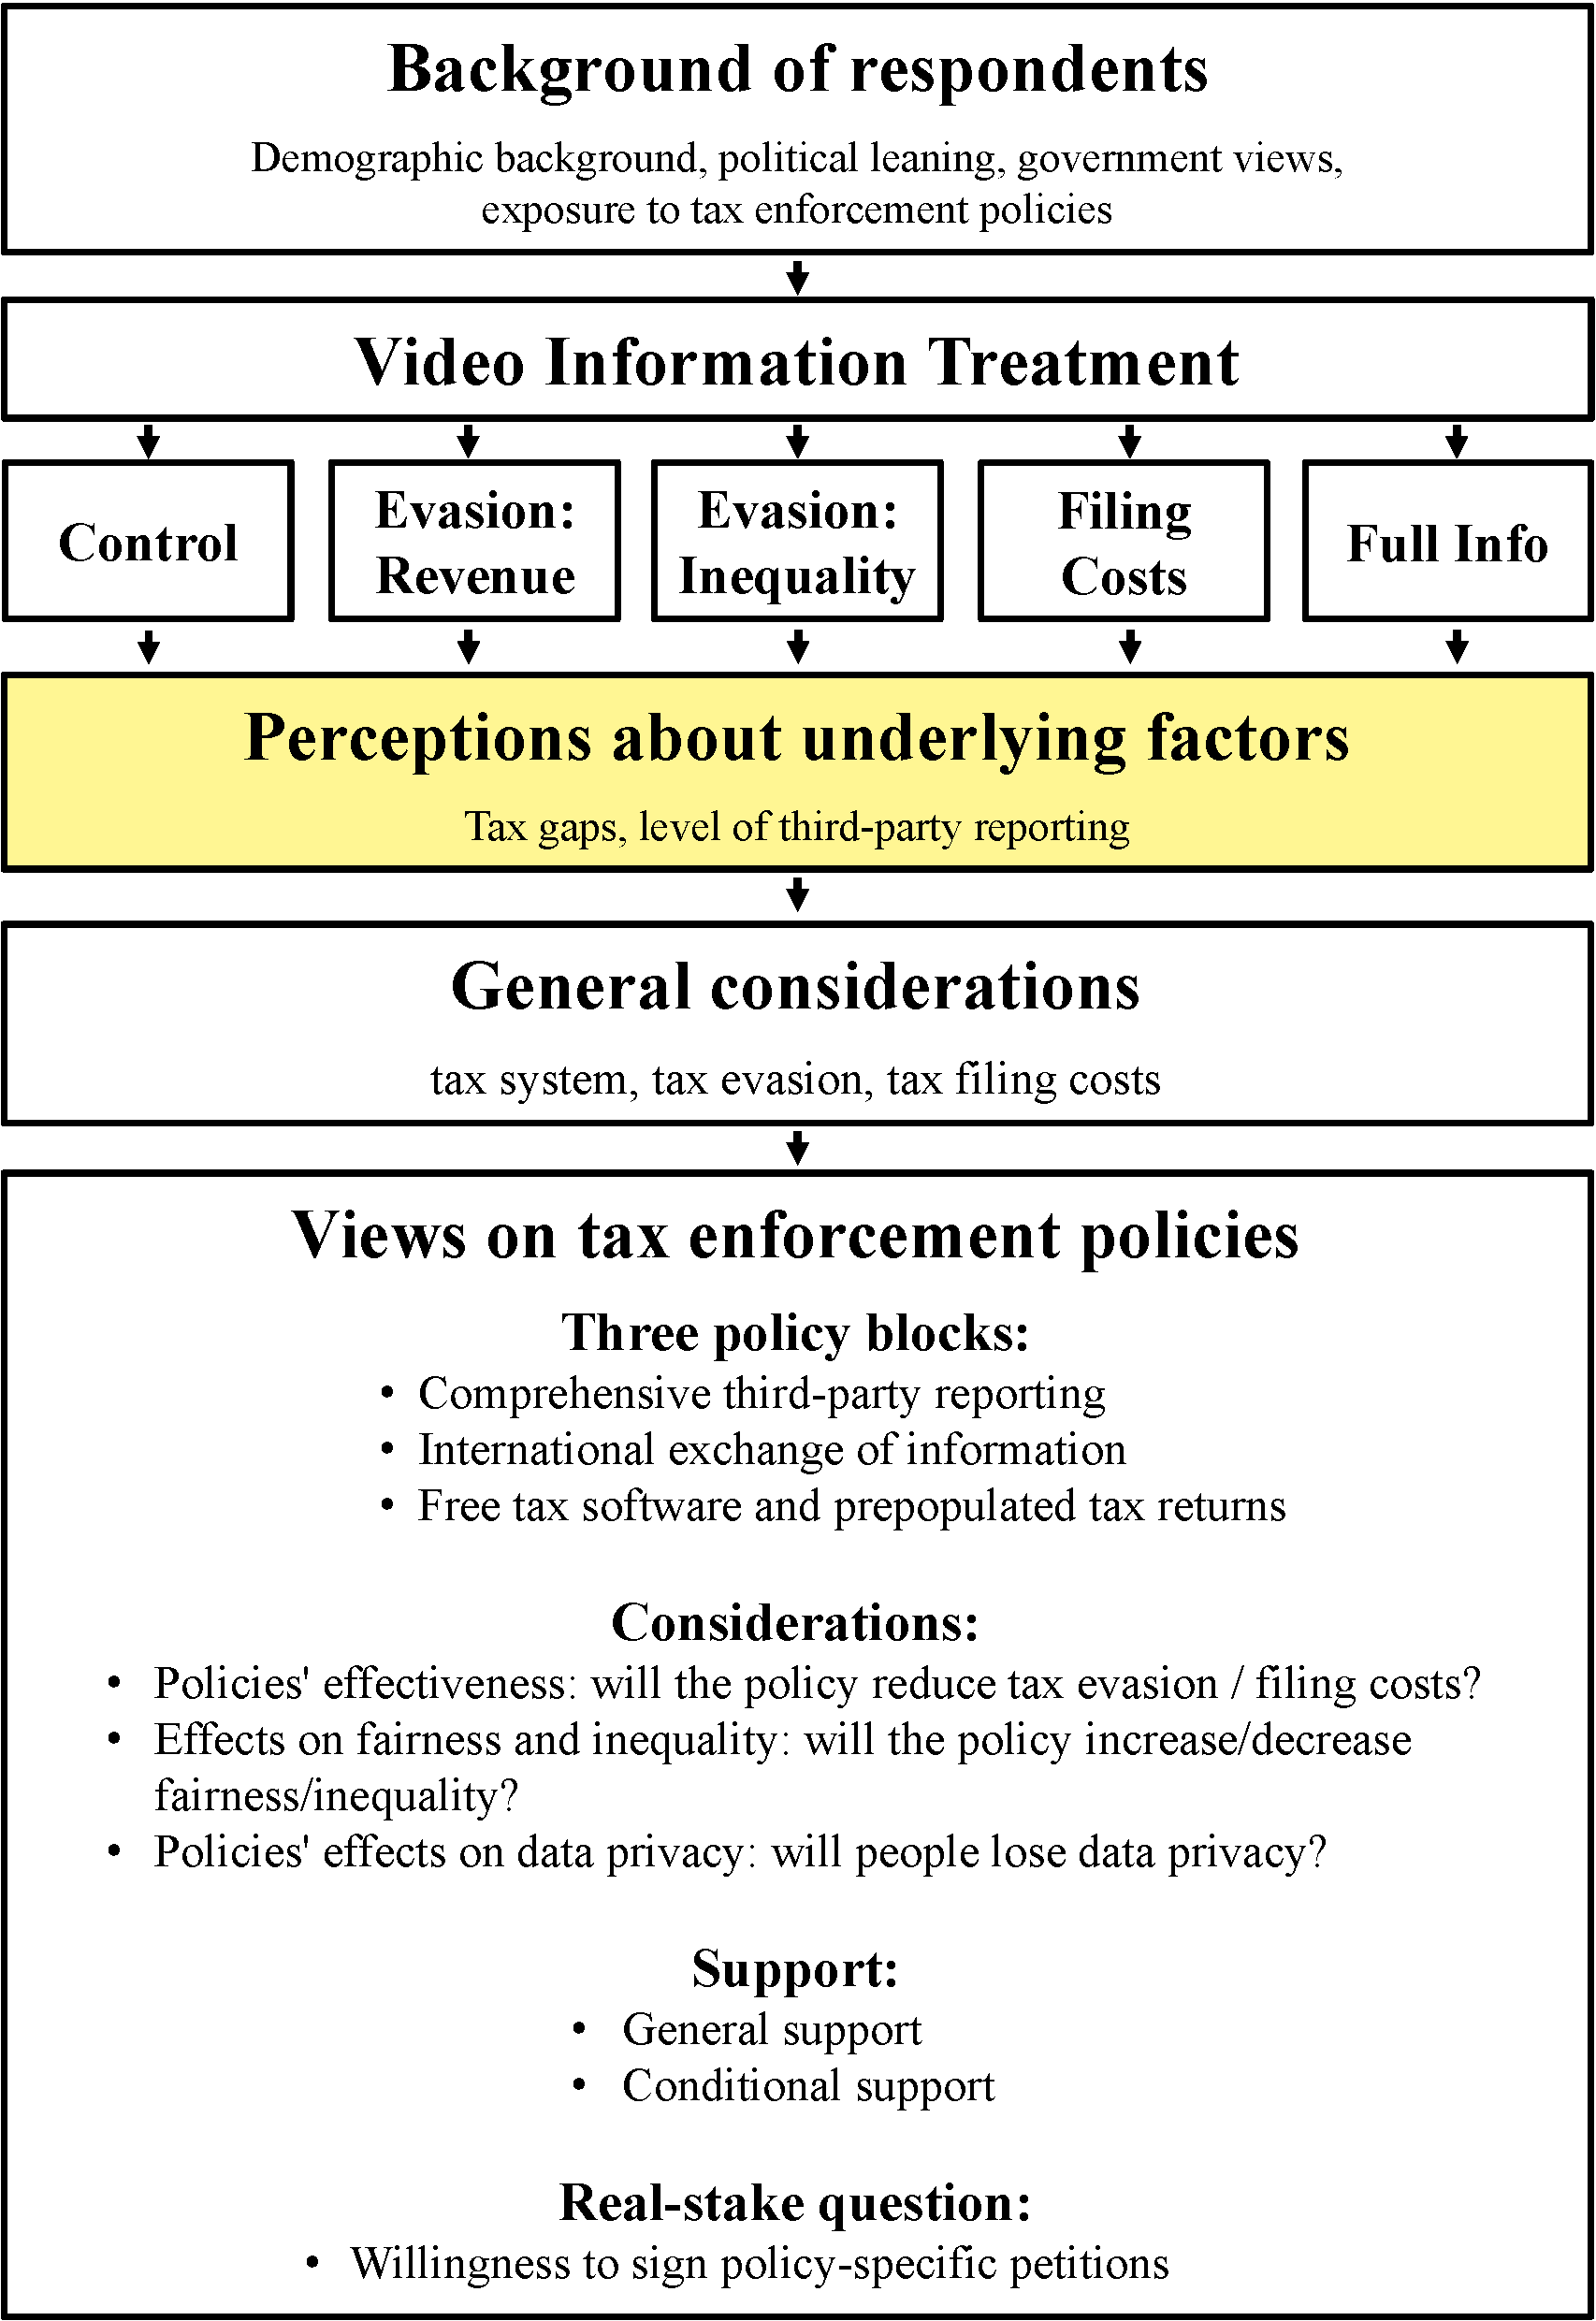
\includegraphics[width=1.05\linewidth]{Figures_Slides/Survey_Overview_Prior.pdf}
%   \end{column}
% \end{columns}
% \end{frame}

% \begin{frame}[label=General_Considerations]{General Considerations \hyperlink{General_Considerations_Appendix}{\beamergotobutton{A: GC}}}
% \begin{columns}[T] % align columns at the top
%   \begin{column}{0.45\textwidth} % left side for text
%     \begin{itemize}
%     \item Tax system 
%     \begin{itemize}
%         \item Is it fair? 
%     \end{itemize}
%     \vspace{0.2em} 
%     \item Tax evasion
%     \begin{itemize}
%         \item Is it concerning? 
%         \item Is it important for the government to reduce it?
%     \end{itemize}
%     \vspace{0.2em} 
%     \item Tax filing costs
%     \begin{itemize}
%         \item Are they concerning? 
%         \item Is it important for the government to reduce them?
%     \end{itemize}
%     \vspace{0.2em} 
%     \item Data privacy
%     \begin{itemize}
%         \item Is it a problem if the government collects data on citizens?
%     \end{itemize}
%     \end{itemize}
%   \end{column}
  
%   \begin{column}{0.45\textwidth} % right side for image
%     \centering
%      \vspace{-2em}     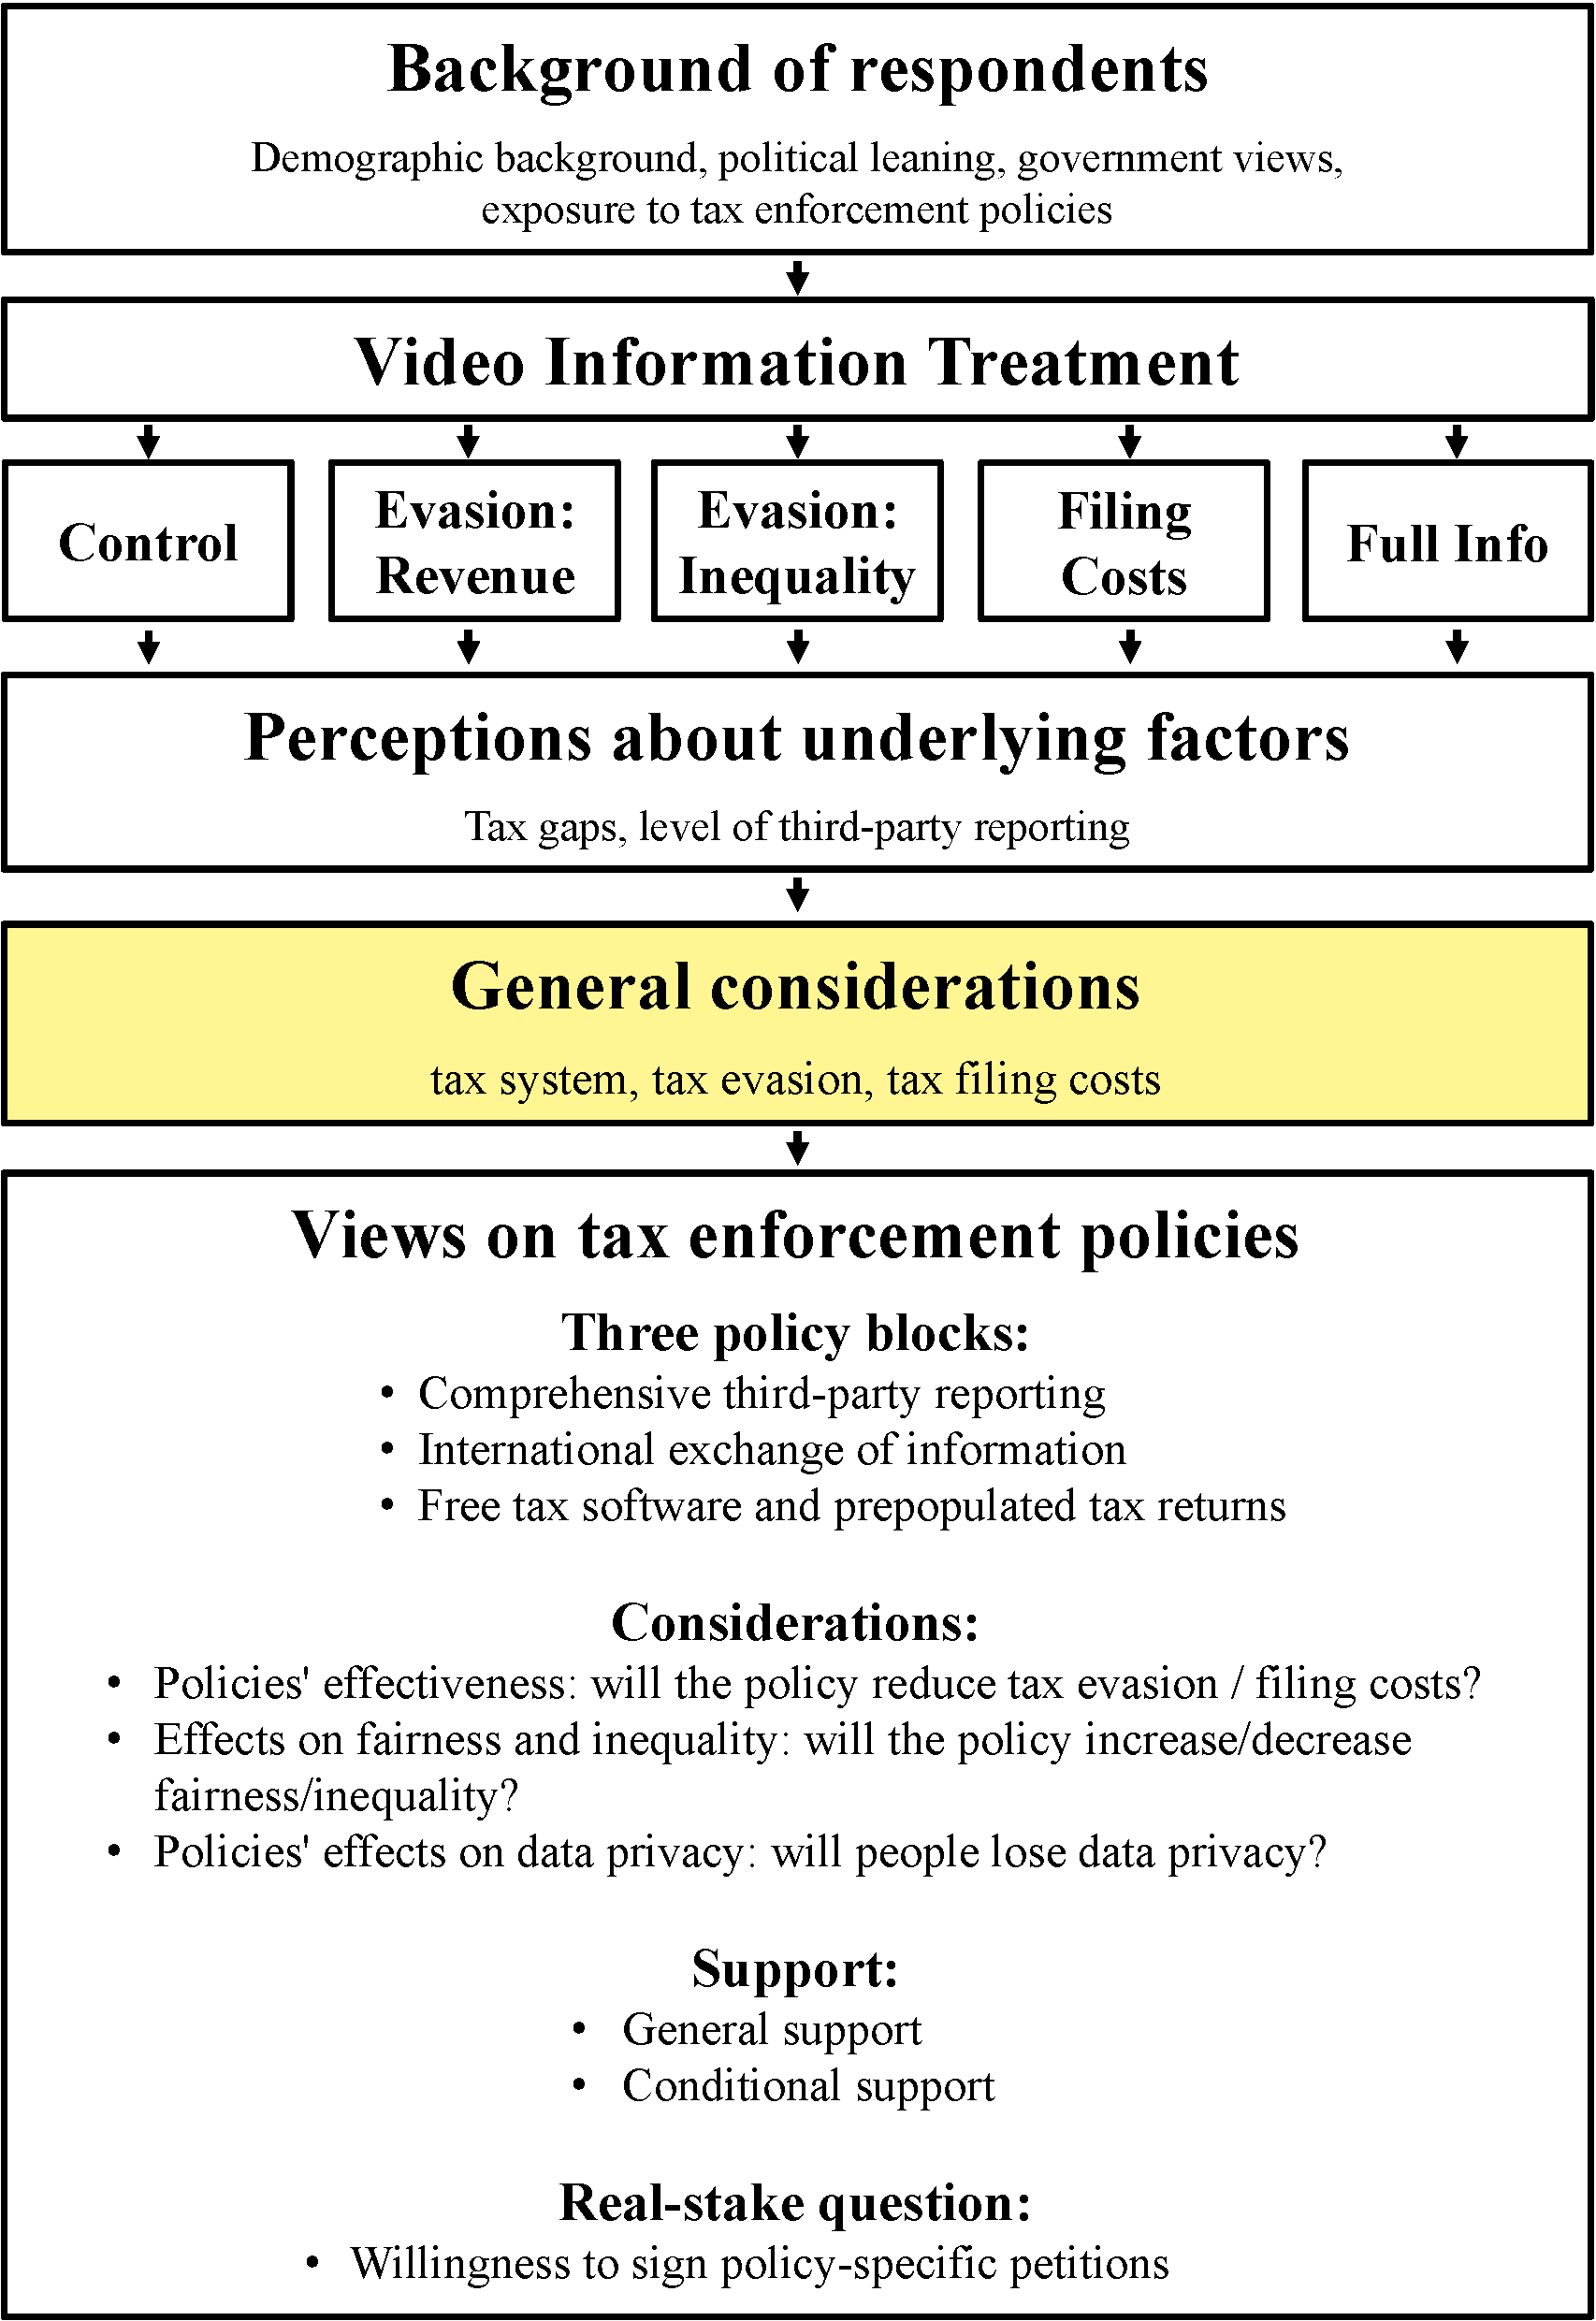
\includegraphics[width=1.05\linewidth]{Figures_Slides/Survey_Overview_General_Considerations.pdf}
%   \end{column}
% \end{columns}
% \hfill
% \vfill
% \end{frame}

% \begin{frame}[label=Third_Party_Reporting]
%   \begin{center}
%  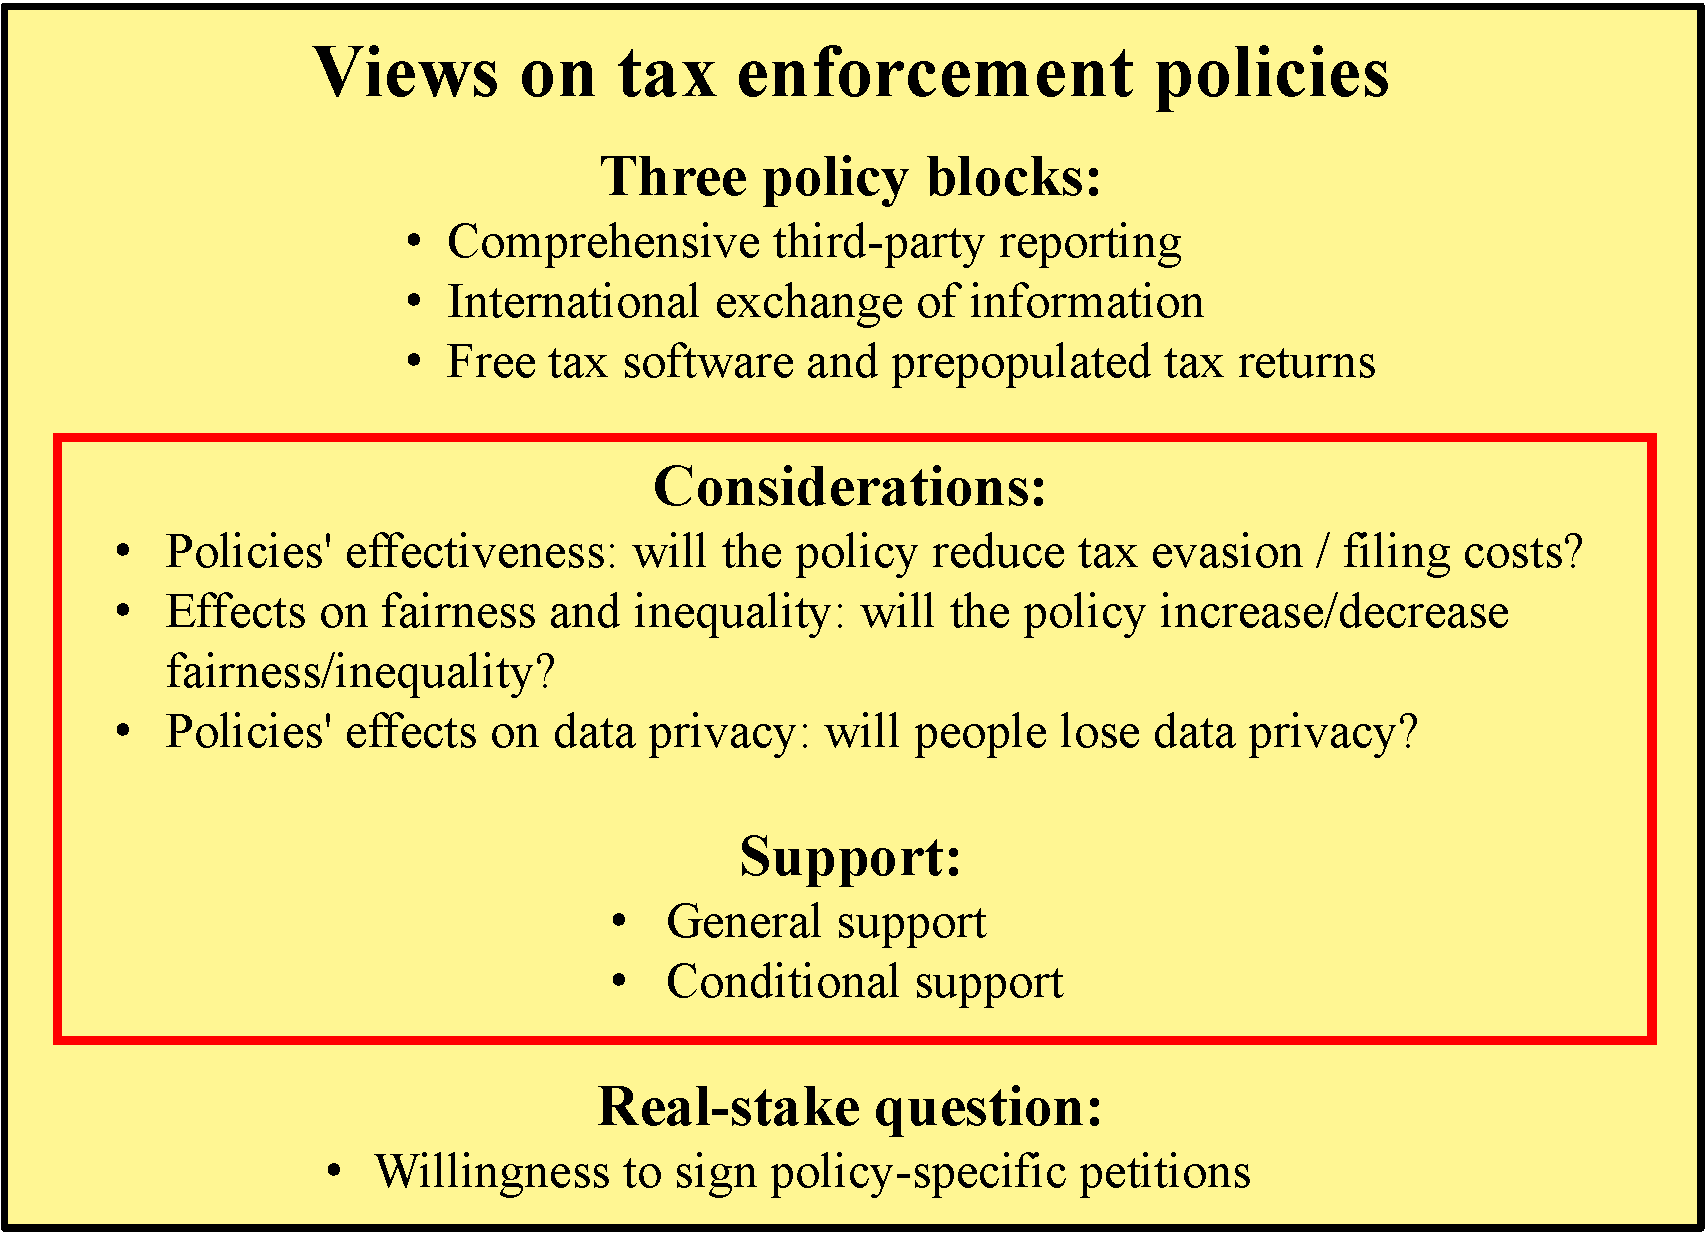
\includegraphics[width=0.65\textwidth]{Figures_Slides/Survey_Overview_Policy_Views_1.pdf} \\
%   \end{center}
%   %\vspace{0.1cm}
%   \begin{center}
%  % <-- Breite nach Wunsch anpassen
% %    The structure of the questionnaire is the same for each policy. \hyperlink{Third_Party_Reporting_Appendix}{\beamergotobutton{A: TPR}}
%     \end{center}
% %     \begin{center}
% % \begin{minipage}{0.65\textwidth}

% %     \begin{enumerate}
% %         \item Short introduction to the policy.
% %         \item Policy-related considerations/expectations.
% %         \item Policy support. (general \& conditional)
% %     \end{enumerate}
% %   \end{minipage}
% %   \end{center}
% \end{frame}




% \begin{frame}[label=Petitions]
%   \begin{center}
%     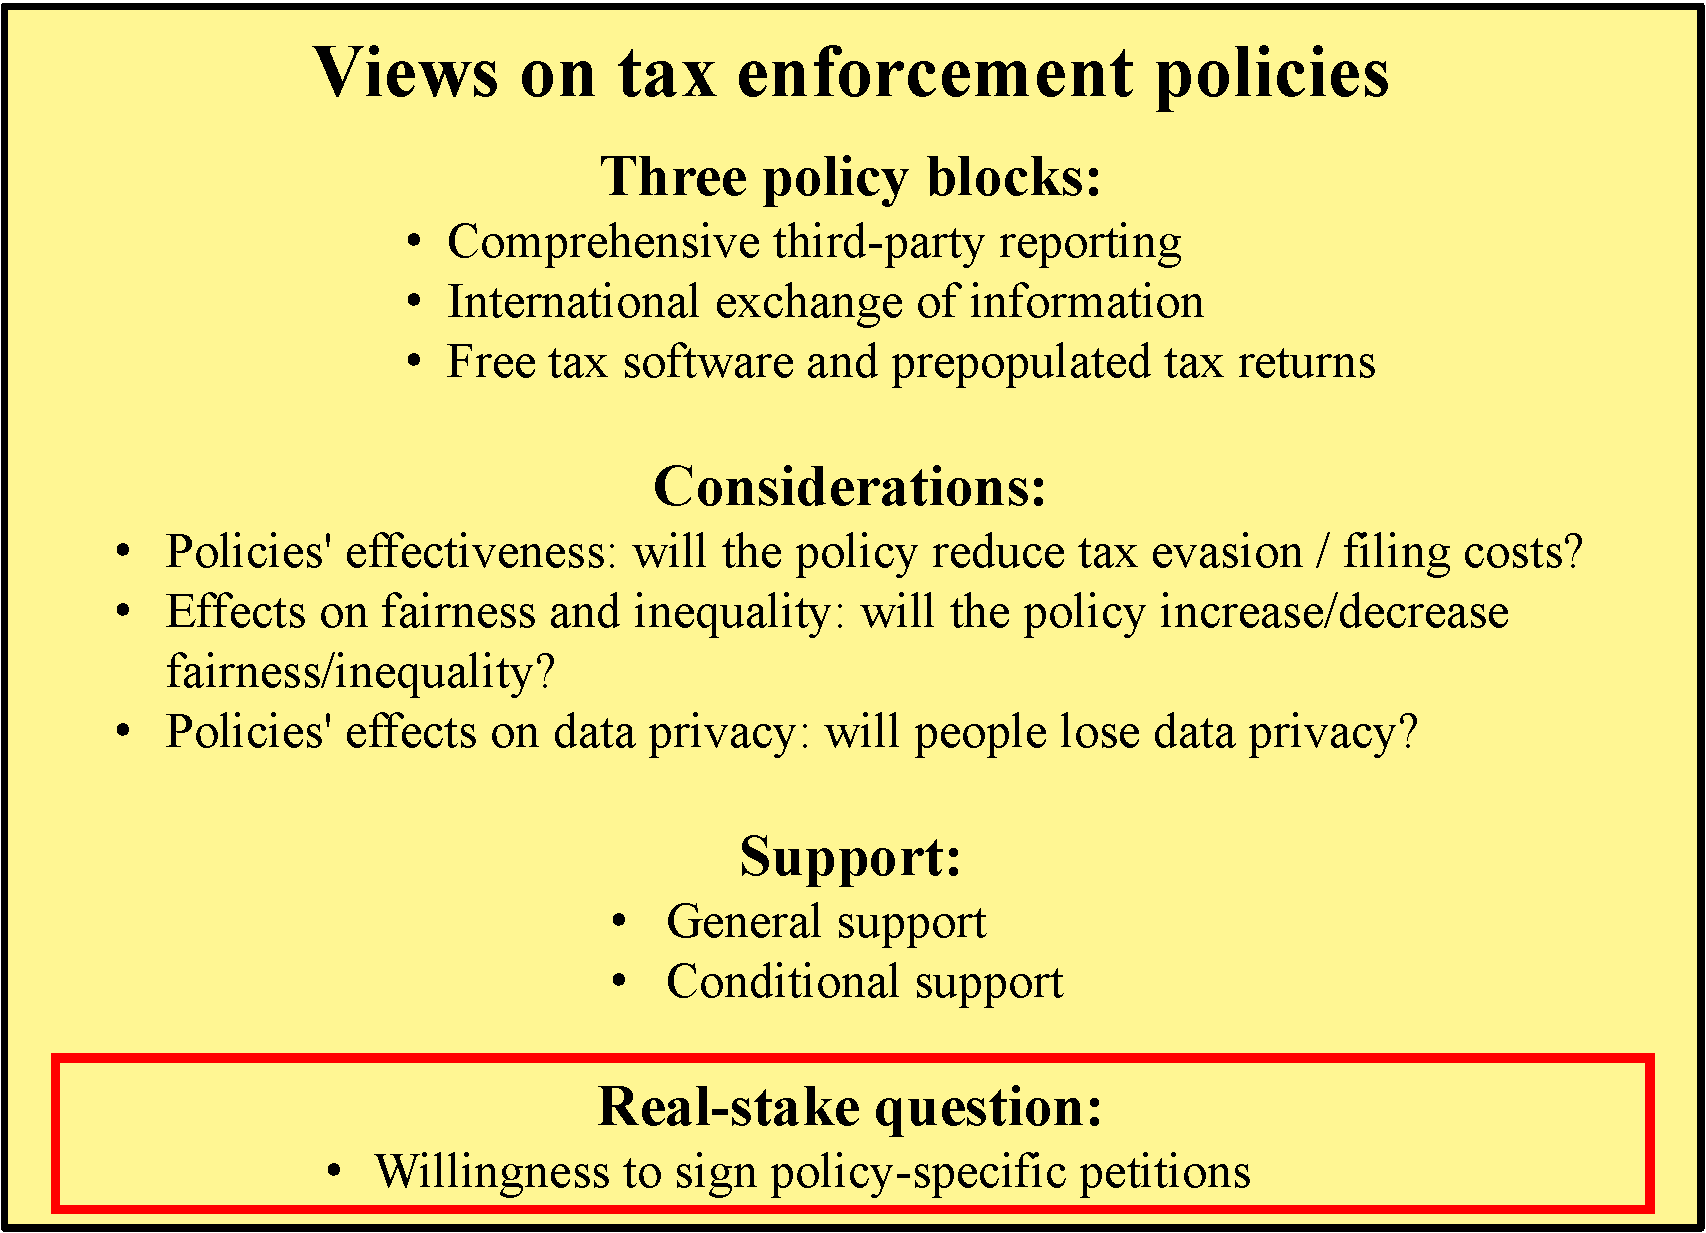
\includegraphics[width=0.65\textwidth]{Figures_Slides/Survey_Overview_Policy_Views_2.pdf} \\
%   \end{center}
% We ask respondents if they want to support \alert{petitions} that aim at policies very similar to our policies from the survey.  \hyperlink{Petitions_Appendix}{\beamergotobutton{A: Petitions}}

%   \footnotesize % make the font smaller only for the table
%   \begin{tabularx}{\textwidth}{*{2}{>{\centering\arraybackslash}X}}
%     \begin{enumerate}
%       %\item TPR$^{+}$ $\times$ \\Tax evasion$^{-}$
%       \item \alert{in favor} of comprehensive \alert{third- party reporting} to act against tax evasion.
%     \end{enumerate} &
%     %\begin{enumerate}
%     %\setcounter{enumi}{1} % start at 2
%     %  %\item TPR$^{-}$ $\times$ \\Data privacy$^{+}$
%     %  \item \alert{against} comprehen- sive \alert{third-party reporting} in order to protect privacy.
%     %\end{enumerate} &
%     \begin{enumerate}
%     \setcounter{enumi}{1} % start at 2
%       %\item Filing services$^{+}$ $\times$ \\Filing costs$^{-}$
%       \item \alert{in favor of making tax filing easier} and more accessible for everyone.
%     \end{enumerate} \\
%   \end{tabularx}
%   \normalsize % reset font size after the table
% \end{frame}

% \begin{frame}{Conclusion}
% \begin{itemize}
% \item Using a survey \alert{we explore peoples' attitudes and considerations towards information-sharing and free tax filing services.} 
% \begin{itemize}
% \item Towards more comprehensive third-party reporting and international automatic exchange of information.
% \item Towards free tax software and/or prepopulated tax returns.
% \end{itemize}
% \vspace{0.5em}
% \item We include questions to \alert{uncover important drivers of policy views.}
% \begin{itemize}
%     \item Perceptions, beliefs and important considerations 
% \end{itemize}
% \vspace{0.5em}
% \item To \alert{establish causal links} between reasoning and policy views, we \alert{experimentally show} people different educational \alert{videos}.
% \end{itemize}
% \end{frame}




 \setbeamertemplate{footline}{} % remove slide numbers
 \setbeamertemplate{navigation symbols}{}

\begin{frame}[noframenumbering,label=thanks]
\centering
\vfill
{\Huge {Thanks for your attention!}} %\\[1.5em]
%{\Large Questions and feedback to:} \\[0.5em]
%\texttt{tim.kircali@unisg.ch}
\vfill
\end{frame}


% \appendix

% \begin{frame}[label=Personal_Exposure_Appendix]
% \frametitle{Appendix: Personal Exposure to Taxes I}
% \footnotesize
% \begin{enumerate}
%     \item People file their tax returns in different ways. Some prepare and submit them on their own, while others rely on help from friends, relatives, or professionals. How do you usually file your taxes?\\ 
%     \textit{(I prepare and file them myself / ... /  ... / ... )}
%     \item Some peoples' tax returns are filed using tax software, while those of others are filed by hand. How are your tax returns filed, by hand or by using tax software? \\ 
%     \textit{(By hand / By using tax software / ... / ... )}
%     \item How tedious do you think that the task of filing taxes is? \\ \textit{(1: Not tedious at all - 10: Very tedious)}
%     \item Many people find parts of the tax system confusing and may unintentionally make mistakes when filing their tax returns. How likely do you think it is that this has ever happened to you?\\
%     \textit{(1: Very unlikely - 10: Very likely) }
%     \item How much would you at most be willing to pay to have your tax return filled in for you, so that you only need to confirm? \\
% \textit{(Slider \$0-\$10000)} \\

% \end{enumerate}
% \end{frame}

% \begin{frame}
% \frametitle{Appendix: Personal Exposure to Taxes II}
% \footnotesize
% For the next three questions, please evaluate how likely you think it is that other people will do certain things when filing their taxes. \uline{When answering these questions, please only consider people you know personally.} 
% \begin{enumerate}
%     \setcounter{enumi}{5}
%     \item How likely do you think it is that people you know personally unintentionally make mistakes in their tax returns ? \\
%     \textit{(1: very unlikely - 10: very likely / Prefer not to say)}
%     \item Some people intentionally report minor details incorrectly to reduce their tax burden. Thinking about people you know personally, how likely do you think it is that they intentionally report minor details incorrectly?\\
%     \textit{(1: very unlikely - 10: very Likely / Prefer not to say)}
%     \item Others may go further and deliberately conceal significant parts of their income to avoid paying higher taxes. Among people you know personally, how likely do you think it is that they hide significant parts of their income to avoid paying higher taxes?\\
%     \textit{(1: very unlikely - 10: very likely / Prefer not to say)}
% \end{enumerate}
% \vfill
% \hfill
% \hyperlink{Personal_Exposure}{\beamergotobutton{Back}}
% \end{frame}

% \begin{frame}[label=Prior_Perceptions_Appendix]
% \frametitle{Appendix: Perceptions about Tax Gaps I}
% \footnotesize
% \noindent Please carefully read the following explanation and keep it in mind when answering the next question. \\
% \vspace{0.5em}
% \begin{adjustwidth}{1em}{1em} \textbf{Explanation:} Some individuals and companies do not pay their taxes fully. They may hide income or assets from the tax authorities, or they may misreport information on their tax returns. This is called tax evasion. Some taxpayers may also make unintentional mistakes when filing tax returns. Due to tax evasion and unintentional mistakes governments collect less tax revenue than they should. 
% \end{adjustwidth}
% \begin{enumerate}
%     \item If you had to take a guess, what percentage of total tax revenue do you think is lost due to tax evasion? \\
%     \textit{(0\% - 100\%)}
% \end{enumerate}
% \end{frame}
% \begin{frame}
% \frametitle{Appendix: Perceptions about Tax Gaps II}
% \footnotesize
% \begin{enumerate}
% \setcounter{enumi}{1}
%     \item Some groups of taxpayers may contribute differently to the missing tax revenue. What do you think, what is the average percentage of taxes evaded by the following groups? (In red you can see the level of tax evasion you indicated before for the overall population.)
%     \begin{itemize}
%         \item Large businesses \textit{(0\% - 100\%)}
%         \item Small businesses \textit{(0\% - 100\%)}
%         \item High-income households \textit{(0\% - 100\%)}
%         \item Middle-income households \textit{(0\% - 100\%)}
%         \item Low-income households \textit{(0\% - 100\%)}
%     \end{itemize}
% \end{enumerate}
% \vfill
% \hfill
% \hyperlink{Prior_Perceptions}{\beamergotobutton{Back}}
% \end{frame}

% \begin{frame}[allowframebreaks]
% \label{General_Considerations_Appendix}
% \frametitle{Appendix: General Considerations}
% \footnotesize
% \begin{enumerate}
%     \item How serious do you consider the issue of income and wealth inequality in your country?\\
%     \textit{(1: Not an issue at all - 10: A very serious issue)}
%     \item How fair do you consider the way your country collects taxes from individuals and businesses?\\
%     \textit{(1: Very unfair – 10: Very fair)}
%     \item In your opinion, how important are taxes as a tool to reduce income and wealth inequality?\\
%     \textit{(1: Not important at all - 10: Very important)}
%     \item Think about the group of people that evade taxes. Do you think that this group is small (which means taxes are evaded only by a small number of people), or do you think the group is large (which means tax evasion is widespread across the population)?\\
%     \textit{(1: Small group of people evade taxes - 10: Tax evasion is widespread across the population)}
%     \item In general, how concerning is the current level of tax evasion in your country?\\
%     \textit{(1: Not concerning at all - 10: Very concerning)}
%     \item Considering all the responsibilities a government has, how important do you think it is that the government ensures all taxes owed are actually paid — for example, by preventing or reducing tax evasion?\\
%     \textit{(1: Not important at all  - 10: Very important)}
% \end{enumerate}

% \noindent Please carefully read the following explanation and keep it in mind when answering the following questions. \\[0.5em]
% \begin{adjustwidth}{1em}{1em} \textbf{Explanation:} Tax filing costs are the costs incurred when filing taxes. These include expenses for software license fees, expenses for paying someone else to file tax returns, but also the time cost when filing the taxes. 
% \end{adjustwidth}
% \begin{enumerate}
%     \setcounter{enumi}{6}
%     \item Do you consider tax filing costs in your country to be low or high?\\ 
%     \textit{(1: Very low - 10: Very high)}
%     \item Considering all the responsibilities a government has, how important do you think it is for the government to try lowering the costs associated with filing taxes? \\ \textit{(1: Not important at all - 10: Very important)}
% \end{enumerate}
% The following question ask about your general views on the federal government. When answering, \uline{please think broadly about the past 10 years and your expectations for the next 10 years, and try to set aside the actions of any specific administration.}

% \begin{enumerate}
%     \setcounter{enumi}{8}
%     \item Some people are concerned about governments automatically collecting data on individuals and businesses, viewing it as a potential threat to privacy. Others believe that such data collection is acceptable or even beneficial if it serves public interests, such as ensuring tax compliance or improving public services. \\ How concerned are you about the government collecting data on individuals and businesses?\\
%     \textit{(1: Not concerned at all - 10: Very concerned)}
% \end{enumerate}
% %\vfill
% \hfill
% \hyperlink{General_Considerations}{\beamergotobutton{Back}}
% \end{frame}

% \begin{frame}[label=Third_Party_Reporting_Appendix]
% \frametitle{Appendix: Policy Views Third-Party Reporting I}
% \footnotesize
% \noindent Please carefully read the following explanation of third-party reporting and keep it in mind when answering the following questions. \\[0.5em]

% \begin{adjustwidth}{1em}{1em}  \textbf{Explanation:} In order to fulfil its functions, the tax authority uses information from other sources, such as employers, banks and insurance companies. With third-party reporting, this tax-relevant data is automatically sent from domestic firms and institutions to the tax authority. In a comprehensive third-party reporting system, the tax authority receives detailed and automatic reports from many sources. \\[0.5em]
% \end{adjustwidth}
% \begin{enumerate}
%     \item Do you think that comprehensive third-party reporting would affect the level of tax evasion? By how much do you think this would reduce the amount of tax evasion (by individuals and businesses?\\
%     \textit{(1: Not reduce tax evasion at all - 10: Strongly reduce tax evasion)}
%     %\item Some people argue that implementing comprehensive third-party reporting would be costly. Others believe that the additional tax revenue it generates would outweigh these costs. In your opinion, would comprehensive third-party reporting lead to a net increase in government revenue (i.e., after subtracting administrative costs), or not? In your opinion, by how much would net revenue increase or decrease?  \\
%     \item In your opinion, would comprehensive third-party reporting lead to an increase in government revenue, or not? By how much would revenue increase?  \\
%     \textit{(1: No increase in government revenue - 10: Strong increase in government revenue)}

% \end{enumerate}
% \end{frame}


% \begin{frame}
% \frametitle{Appendix: Policy Views Third-Party Reporting II}
% \footnotesize
% \begin{enumerate}
%     \setcounter{enumi}{2}
%     \item Do you think that comprehensive third-party reporting would increase the overall fairness of the tax system?\\
%     \textit{(1: No increase of fairness at all - 10: Strong increase of fairness)}
%     \item In your view, is comprehensive third-party reporting important to reduce income and wealth inequality?\\
%     \textit{(1: Not important at all - 10: Very important)}
%     %\item In your view, to what extent does comprehensive third-party reporting reduce the administrative costs of tax enforcement for the government?\\
%     %\textit{(1: No reduction at all - 10: Strong reduction)}
%     \item To what extent do you think comprehensive third-party reporting helps reduce time and monetary costs for taxpayers when filing their taxes?\\
%     \textit{(1: No reduction at all - 10: Strong reduction)}
%     \item In your opinion, how much privacy do people and businesses lose with comprehensive third-party reporting relative to a tax system with no third-party reporting?\\
%     \textit{(1: No loss of privacy at all - 10: Very strong loss of privacy)}
%     \item How concerning would you find a loss of privacy due to comprehensive third-party reporting?\\
%     \textit{(1: Not concerning at all - 10: Very concerning)}
% \end{enumerate}
% \vfill
% \hfill 
% \hyperlink{Third_Party_Reporting}{\beamergotobutton{Back}}
% \end{frame}

% \begin{frame}[label=Petitions_Appendix]
% \frametitle{Appendix: Petitions}
% \footnotesize
%     Thanks for participating in the survey. For interested respondents we have prepared two related petitions that you can support: 
%     \begin{itemize}
%         \item Petition 1) is in favor of comprehensive third-party reporting to act against tax evasion. 
%         %\item Petition b) is against comprehensive third-party reporting in order to protect privacy and government overreach in the tax system. 
%         \item Petition 2) is in favor of making tax filing easier and more accessible for everyone. 
%     \end{itemize}
%     As soon as the survey is complete, we will send the results to the [head of state’s] office, informing them what share of people who took this survey were willing to support which petition. \\ 
%     \vspace{0.5em} 
%     Would you like to have a look at the petitions to see if you want to support one or more of them? (You will \underline{NOT} be asked to sign, only your answer here is required and remains anonymous.)\\ 
% \vspace{0.5em} 
% \textit{(Yes, I want to look at them / No, I do not want to look at them)} 
% \vfill
% \hfill 
% \hyperlink{Petitions}{\beamergotobutton{Back}}
% \end{frame}







% \begin{frame}[noframenumbering,allowframebreaks]
%   \frametitle{Literature}
%   \printbibliography
% \end{frame}



%----------------------------------------------------------------------------------------
\end{document} 